In this section, we examine the differences between quark- and
gluon-initiated jets in terms of substructure variables. At a fundamental level, the primary difference between quark-  and gluon-initiated jets is the color charge of the initiating parton, typically expressed in terms of the
ratio of the corresponding Casimir factors $C_F/C_A = 4/9$.  
%Since the quark has the smaller color charge, it radiates less than a corresponding
%gluon and the resulting jet will contain fewer constituents. 
Since the quark has the smaller color charge, it radiates less than a
corresponding
gluon and the naive expectation is that the resulting quark jet will contain
fewer constituents than the corresponding gluon jet. The differing color
structure of the two types of jet will also be realized in the detailed
behavior of their radiation patterns.  
We determine the extent to which the substructure observables capturing these differences are correlated, 
providing some theoretical understanding of these
variables and their performance. 
The motivation for these studies
arises not only from the
desire to ``tag'' a jet as originating from a quark or gluon, but also
to improve our  understanding of the quark and gluon components of the
QCD backgrounds relative to boosted resonances.  While recent studies
have suggested that quark/gluon tagging efficiencies depend highly on
the Monte Carlo generator used \cite{Aad:2014gea,Gallicchio:2012ez}, we are more interested in
understanding the scaling performance with $\pt$ and $R$, and the
correlations between observables, which are expected to be treated
consistently within a single shower scheme.

Other examples of recent analytic studies of the correlations between jet observables
relevant to quark jet versus gluon jet discrimination can be found in
\cite{Larkoski:2013paa, Larkoski:2014tva, Larkoski:2014pca, Procura:2014cba}.

\subsection{Methodology and Observable Classes}

%{\it Start adding outline/discussion of theoretical understanding}
These studies use the $qq$ and $gg$ MC samples described  in Section~\ref{sec:samples}. 
The showered events were clustered with \textsc{FastJet}
3.03 using
the \antikt~algorithm with jet radii of $R = 0.4,\, 0.8,\, 1.2$. In
both signal (quark) and background (gluon) samples, an upper and lower cut on
the leading jet $\pt$ is applied after showering/clustering, to ensure
similar $\pt$ spectra for signal and background in each \pt bin. The bins
in leading jet \pt that are considered are 300-400 GeV, 500-600 GeV,
1.0-1.1 TeV, for the 300-400 GeV, 500-600 GeV,
1.0-1.1 TeV parton \pt slices respectively. 
Various jet grooming approaches are applied to the jets, as described in Section~\ref{sec:substructure}. 
Only leading and subleading jets in each sample are used. The
following observables are studied in this section:
%
\begin{itemize}
\item Number of constituents ($n_{\rm constits}$) in the jet.
\item Pruned Qjet mass volatility, $\Gamma_{\rm Qjet}$.
\item 1-point energy correlation functions, $C_1^{\beta}$ with $\beta=0,\,1,\,2$.
\item 1-subjettiness, $\tau_1^{\beta}$ with $\beta=1,\,2$. The $N$-subjettiness axes are computed using one-pass $k_t$ axis optimization.
\item Ungroomed jet mass,  $m$.
\end{itemize}
%
For simplicity, we hereafter refer to quark-initiated jets (gluon-initiated jets) as quark jets (gluon jets).

We will demonstrate that, in terms of their jet-by-jet correlations and their ability to separate quark jets from gluon jets, 
the above observables fall into five Classes.  The first three observables, $n_{\rm constits}$, 
$\Gamma_{\rm Qjet}$ and $C_1^{\beta=0}$, each constitutes a Class of its own  (Classes I to III) in the sense that they each carry some independent information 
about a jet and, when combined, provide substantially better quark jet and gluon jet separation than any one observable alone.  Of the remaining
observables, $C_1^{\beta=1}$ and $\tau_1^{\beta=1}$ comprise a single class (Class IV) because their distributions are  similar 
for a sample of jets, their jet-by-jet values are highly correlated, and they exhibit very similar power to separate 
quark jets and gluon jets (with very similar dependence on the jet parameters $R$ and $p_T$); this separation power is not improved
when they are combined.  The fifth class (Class V) is composed of $C_1^{\beta=2}$, $\tau_1^{\beta=2}$ and the (ungroomed) jet mass.  Again the 
jet-by-jet correlations are strong (even though the individual observable distributions are somewhat different), the quark versus gluon separation power is very similar
(including the $R$ and $p_T$ dependence), and little is achieved by combining more than one of the Class V observables.  This class structure is
not surprising given that the observables within a class exhibit very similar dependence on the kinematics of the underlying jet constituents.%, and we provide more  details below.     
For example, the members of Class V are constructed from of a sum over pairs of constituents using products of the energy of each member 
of the pair times the angular separation squared for the pair (this is apparent for the ungroomed mass when viewed in terms of a mass-squared with small angular separations).  
By the same argument, the Class IV and Class V observables will be seen to be more similar than any other pair of classes, differing only in the
power ($\beta$) of the dependence on the angular separations, which  produces small but detectable differences.  
We will return to
 a more complete discussion of jet masses in Section~\ref{sec:qg_mass}.


\subsection{Single Variable Discrimination}


%Figure~\ref{fig:qg_pt500_mass_AKt_R08} shows the mass of jets in the quark and gluon samples when using
%different groomers, and the ungroomed jet mass, for jets with
%R=0.8 and in the $\pt=500-600 \GeV$ bin. 
%\begin{figure*}
%\centering
%\subfigure[Ungroomed mass]{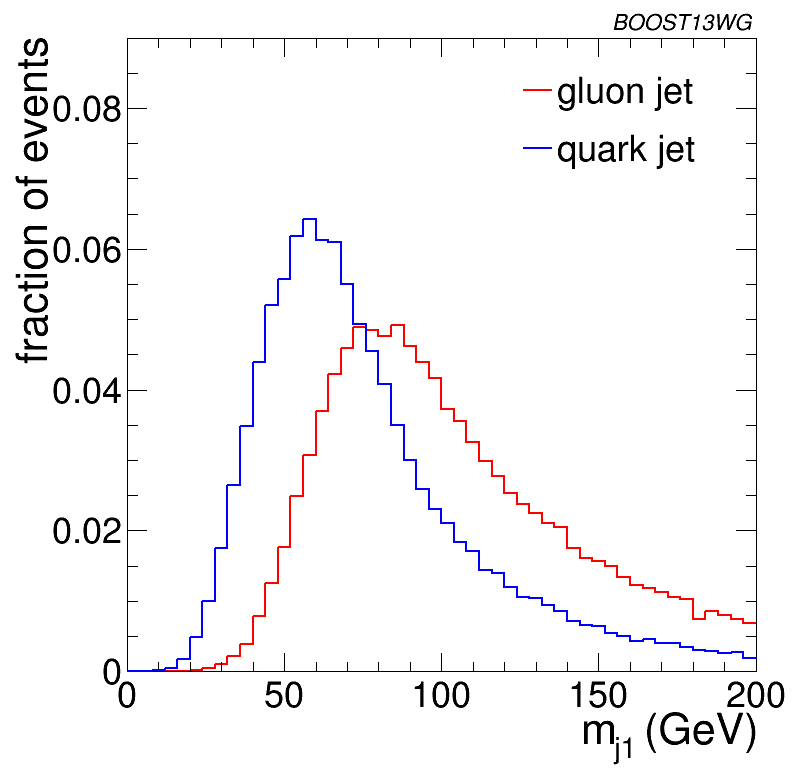
\includegraphics[width=0.30\textwidth]{./Figures/QGTagging/pT500/AKtR08/jmass1.png}}
%\subfigure[Pruned mass]{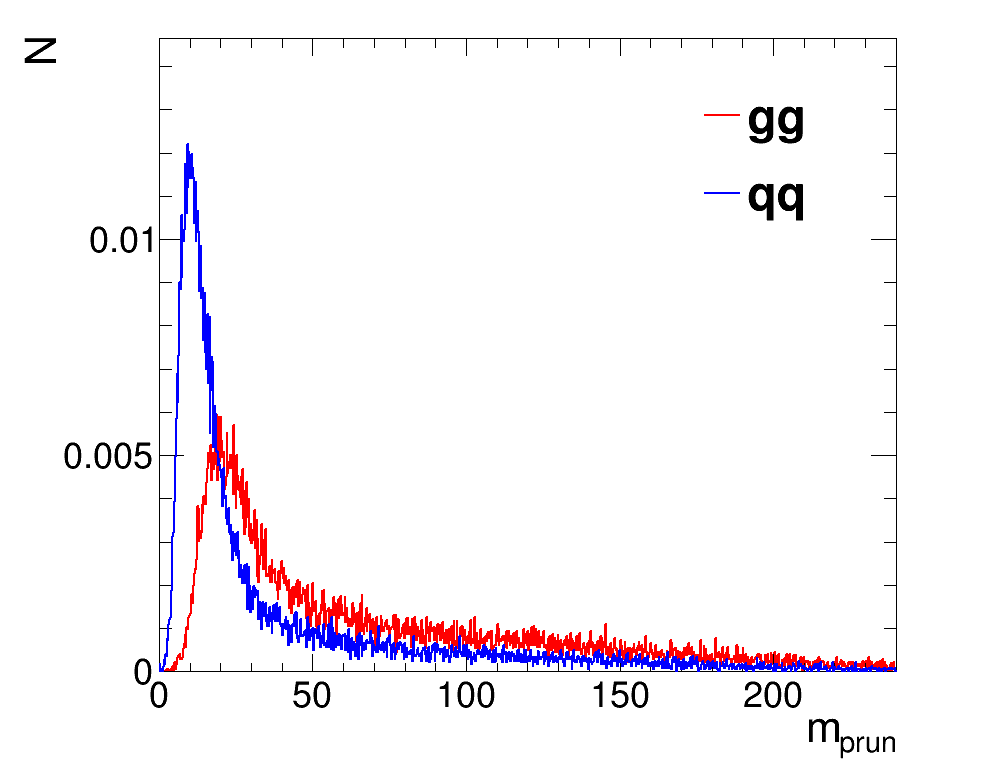
\includegraphics[width=0.30\textwidth]{./Figures/QGTagging/pT500/AKtR08/h_mass_prun.png}}
%\subfigure[Trimmed mass]{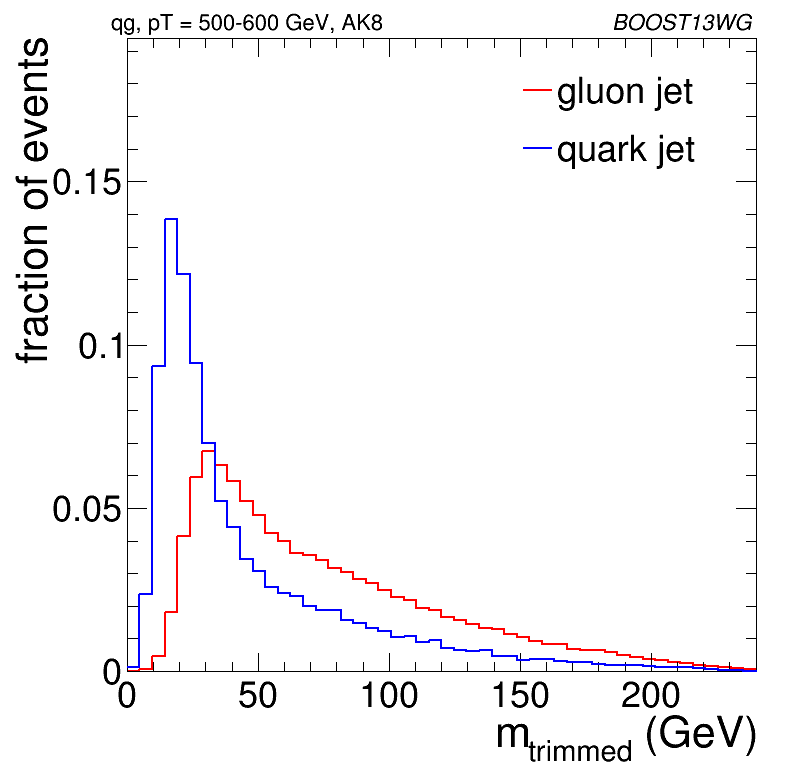
\includegraphics[width=0.30\textwidth]{./Figures/QGTagging/pT500/AKtR08/h_mass_trim.png}}\\
%\subfigure[mMDT mass]{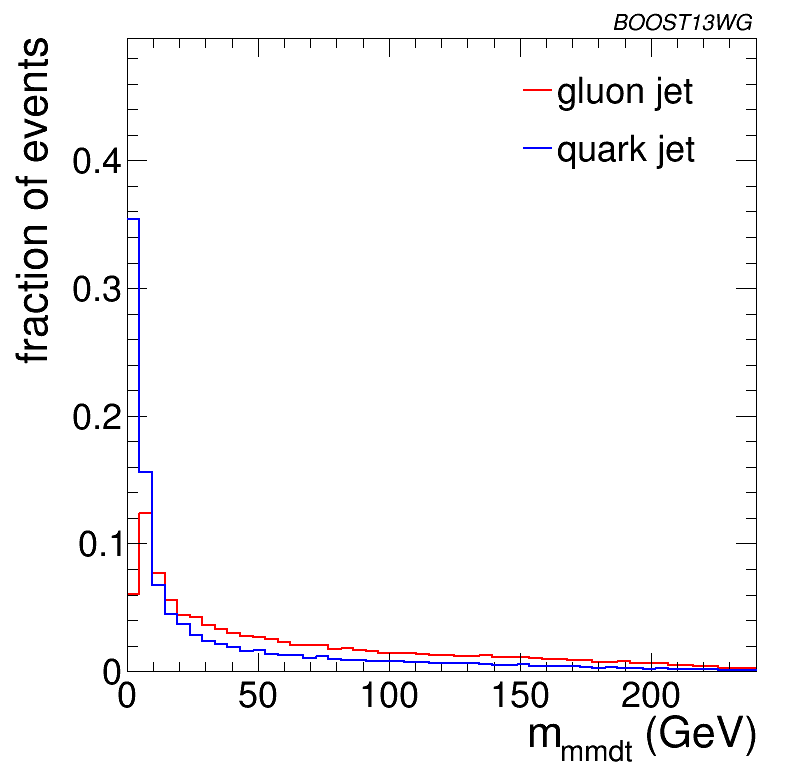
\includegraphics[width=0.30\textwidth]{./Figures/QGTagging/pT500/AKtR08/h_mass_mmdt.png}}
%\subfigure[Soft-drop $\beta=2$ mass]{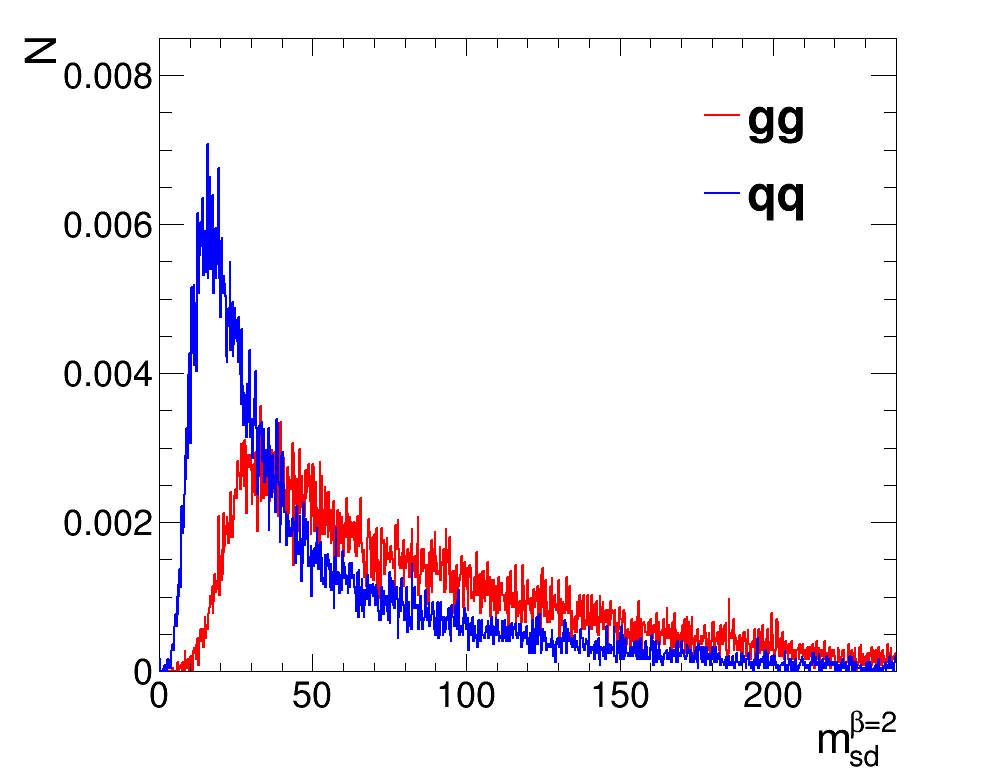
\includegraphics[width=0.30\textwidth]{./Figures/QGTagging/pT500/AKtR08/h_mass_sdb2.png}}
%\subfigure[Soft-drop $\beta=-1$ mass]{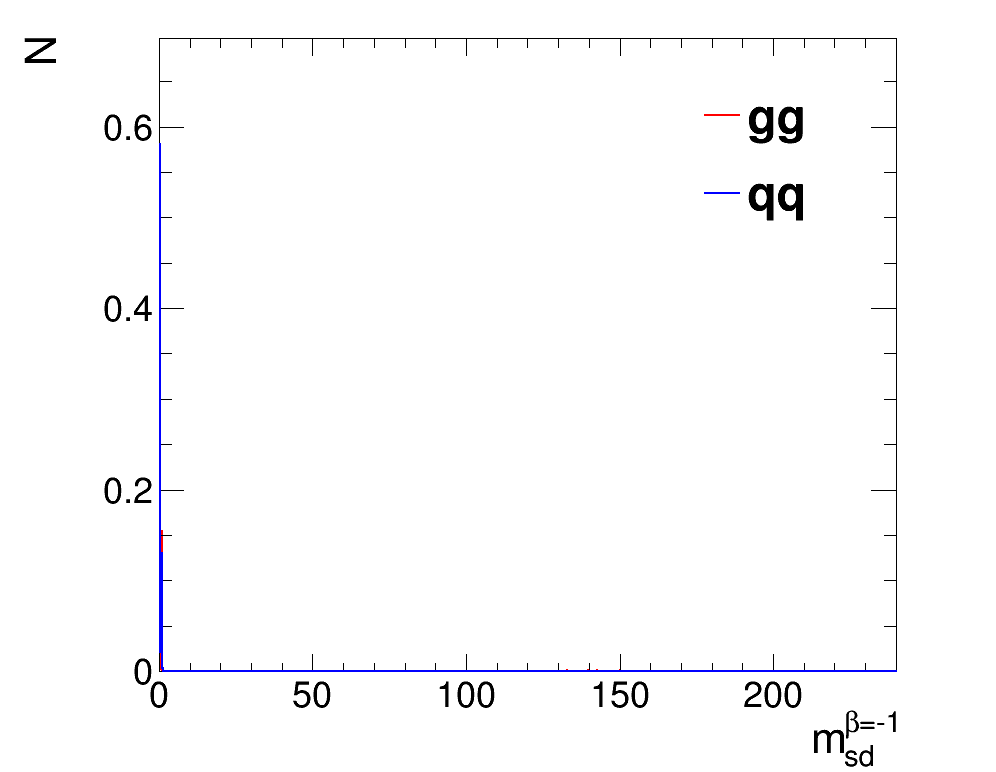
\includegraphics[width=0.30\textwidth]{./Figures/QGTagging/pT500/AKtR08/h_mass_sdm1.png}}
%\caption{Comparisons of ungroomed and groomed quark and gluon mass distributions for leading jets in the 
%$\pt=500-600 \GeV$ bin using the anti-\kT R=0.8 algorithm. }
%\label{fig:qg_pt500_mass_AKt_R08}
%\end{figure*}
%Qualitatively, the application of grooming shifts the mass distributions towards
%lower values when compared to the ungroomed mass, as expected. No clear gain in discrimination can be seen, and for
%certain grooming parameters, such as the use of soft drop with $\beta=-1$ a clear
%loss in discrimination power is observed; this is because the soft-drop condition for $\beta=-1$ discards collinear radiation, and the differences between quarks %and gluons are manifest in the collinear structure (spin, splitting functions, etc.). 


\begin{figure*}
\centering
\subfigure[$n_ {\rm constits}$]{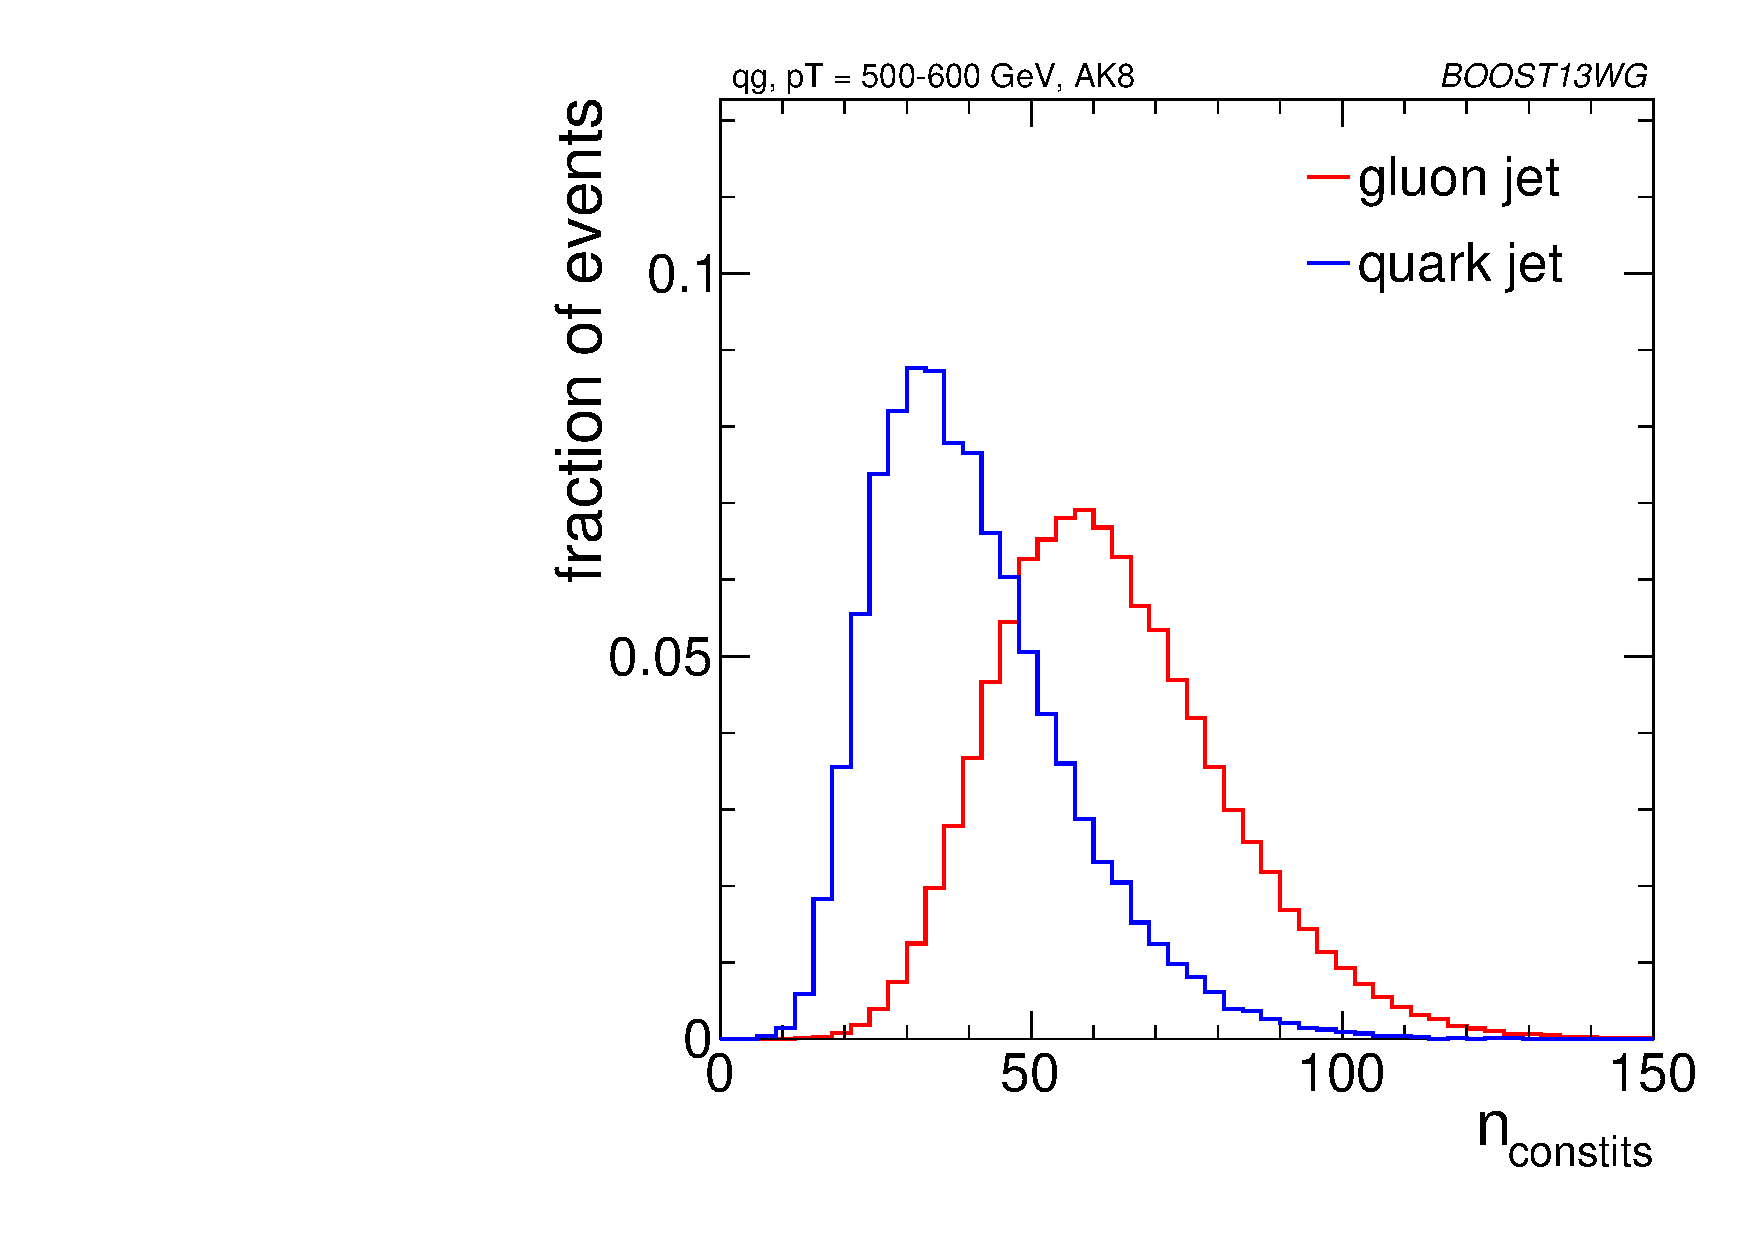
\includegraphics[width=0.30\textwidth]{./Figures/QGTagging/pT500/AKtR08/h_multiplicity.pdf}}
\subfigure[$\Gamma_{\rm Qjet}$]{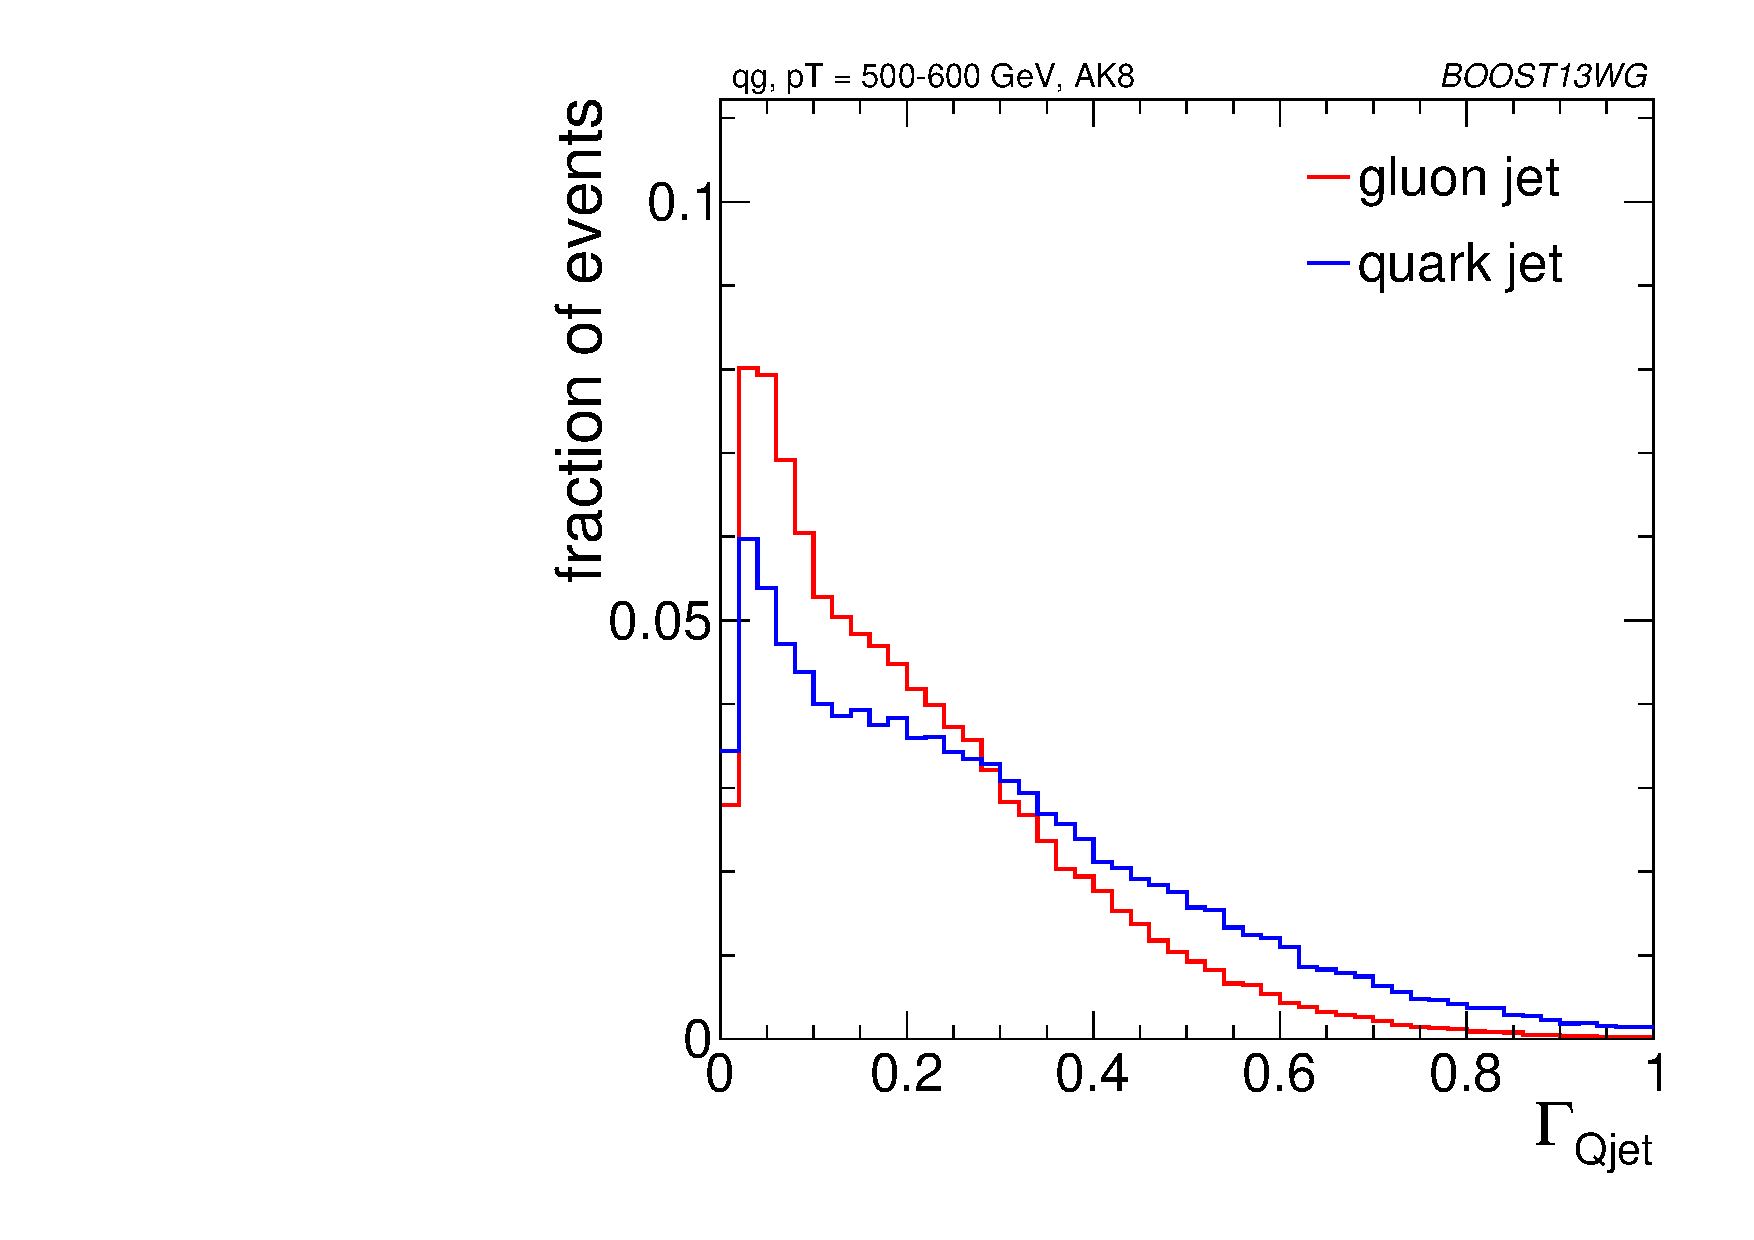
\includegraphics[width=0.30\textwidth]{./Figures/QGTagging/pT500/AKtR08/h_qjetVol.pdf}}
\subfigure[$C_1^{\beta=0}$]{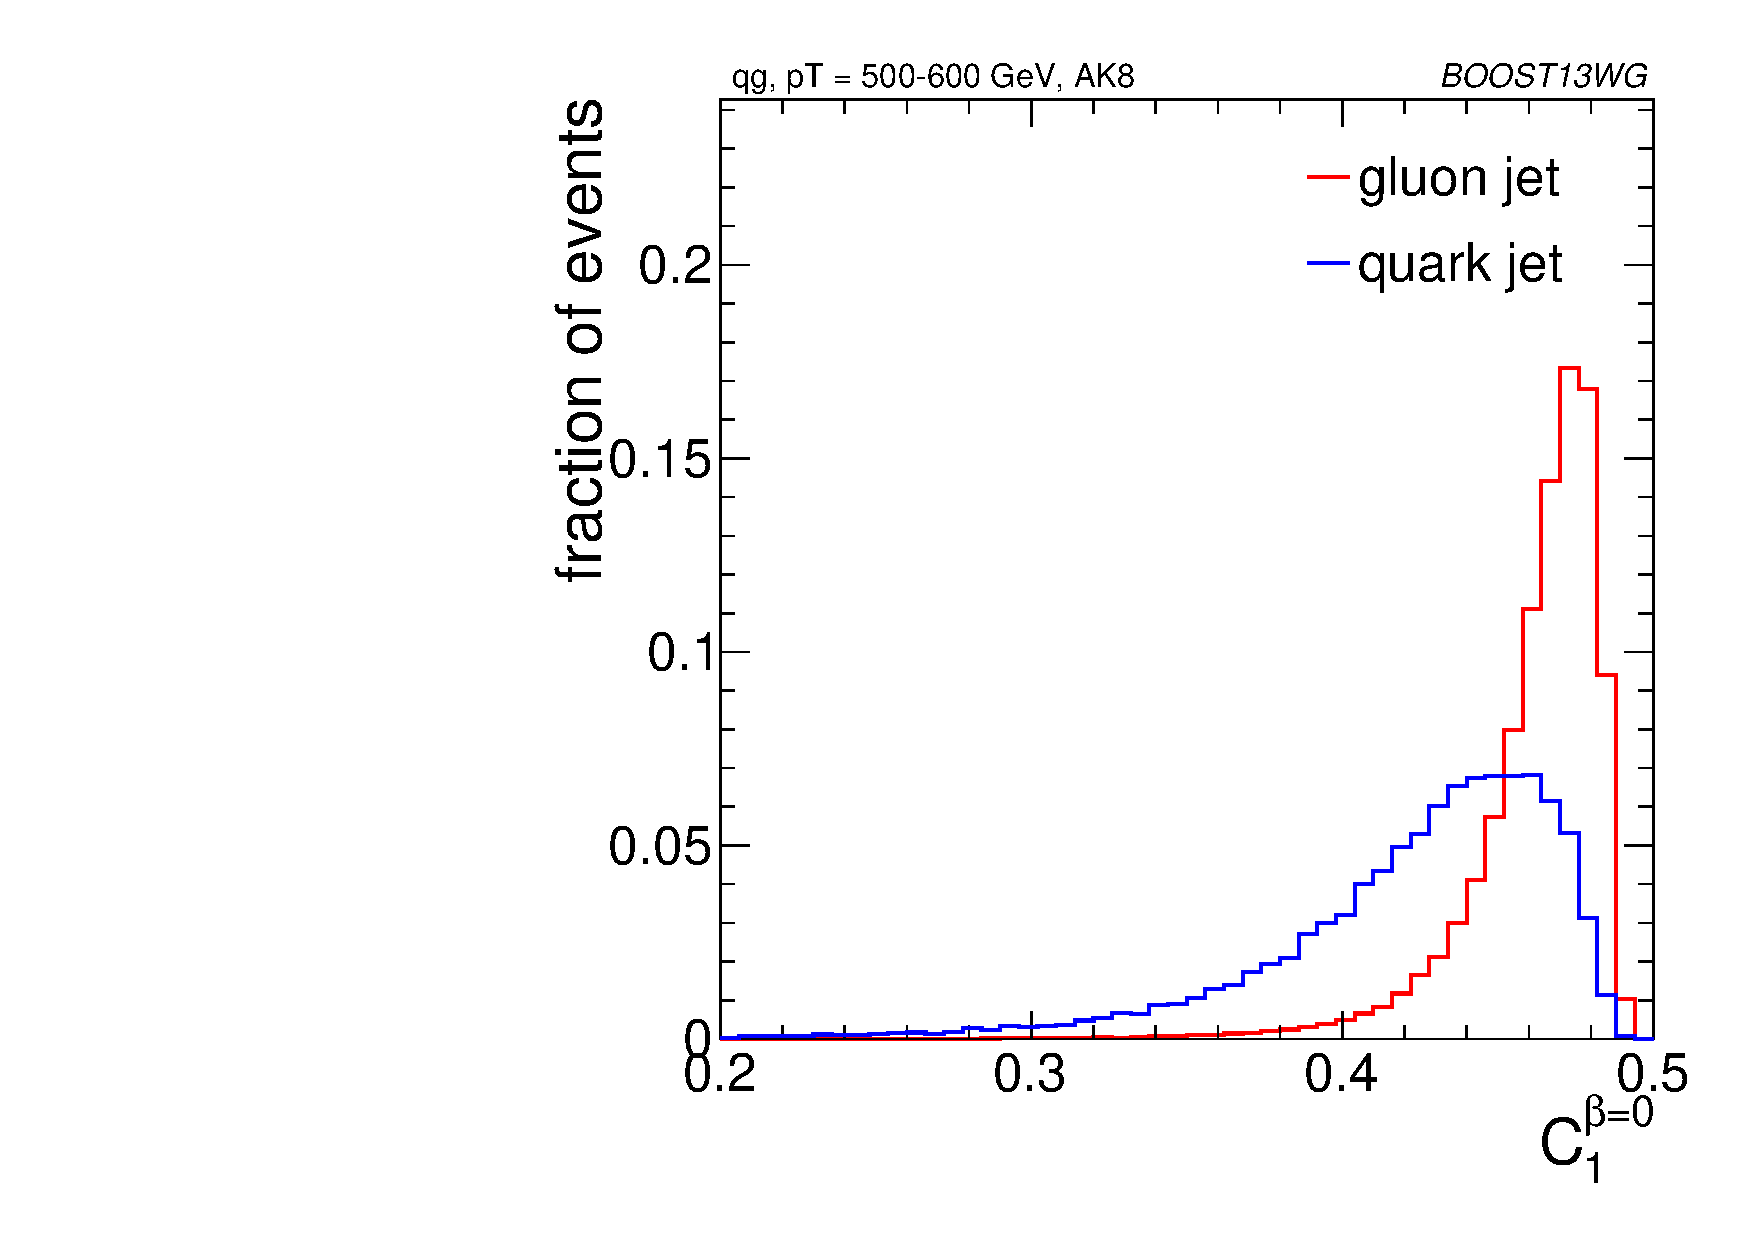
\includegraphics[width=0.30\textwidth]{./Figures/QGTagging/pT500/AKtR08/h_c1_b0.pdf}}\\
\subfigure[$C_1^{\beta=1}$]{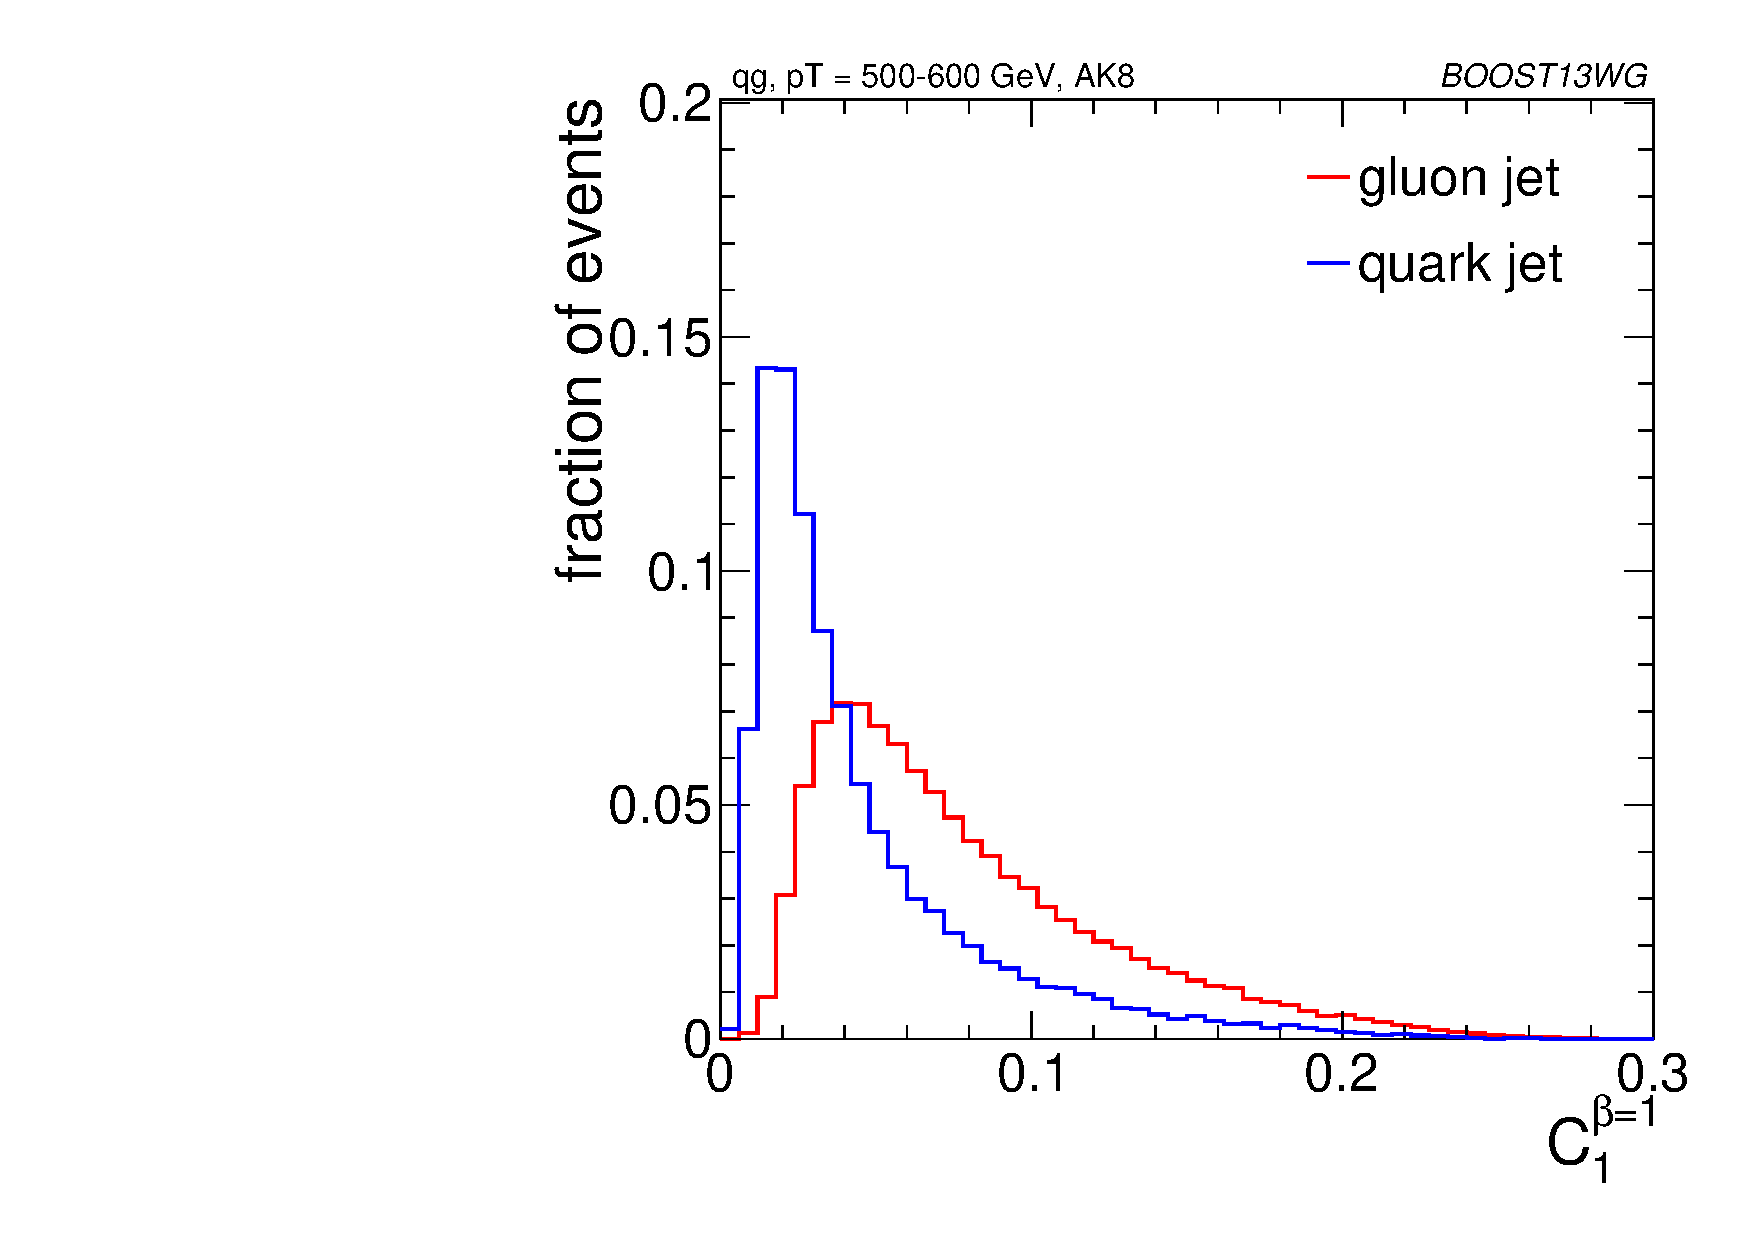
\includegraphics[width=0.30\textwidth]{./Figures/QGTagging/pT500/AKtR08/h_c1_b1.pdf}}
\subfigure[$\tau_{1}^{\beta=1}$]{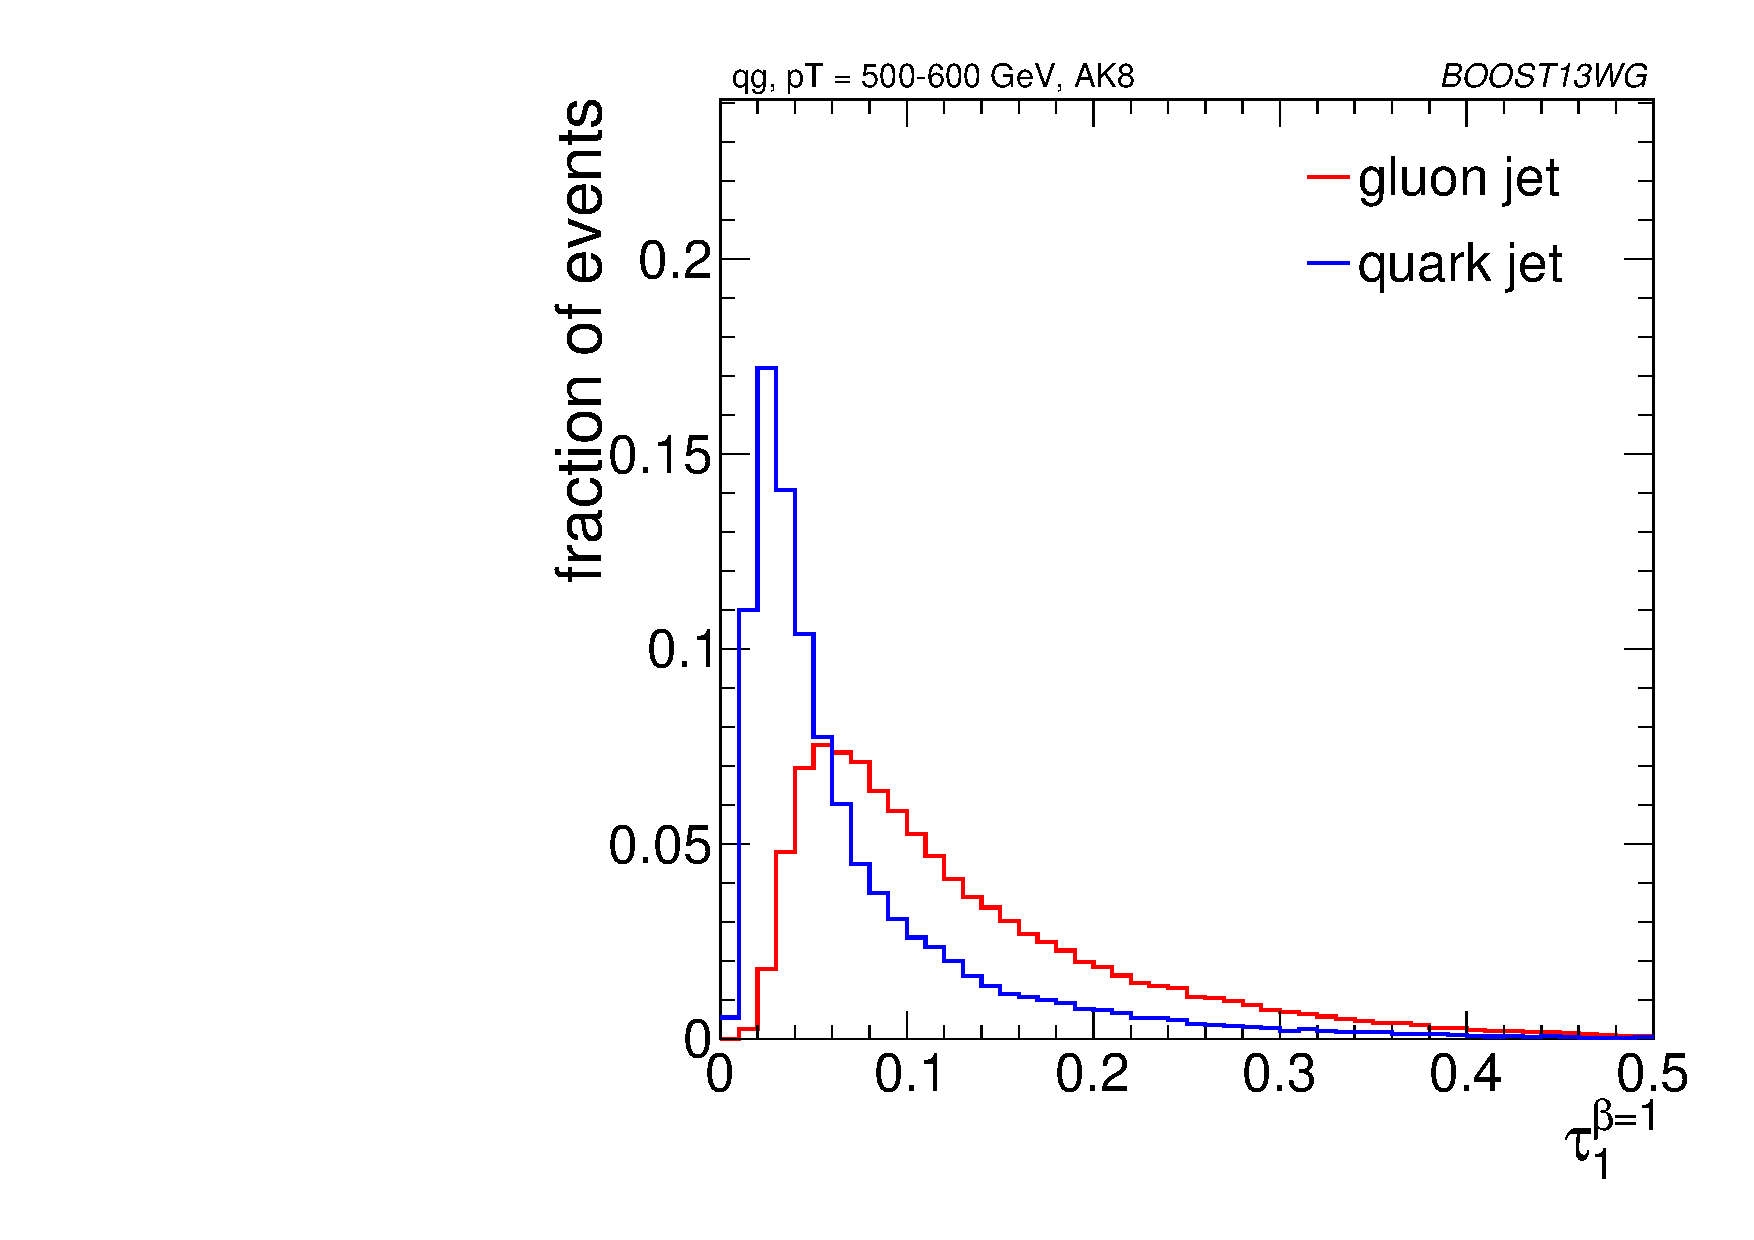
\includegraphics[width=0.30\textwidth]{./Figures/QGTagging/pT500/AKtR08/h_tau1_b1.pdf}}\\
\subfigure[$C_1^{\beta=2}$]{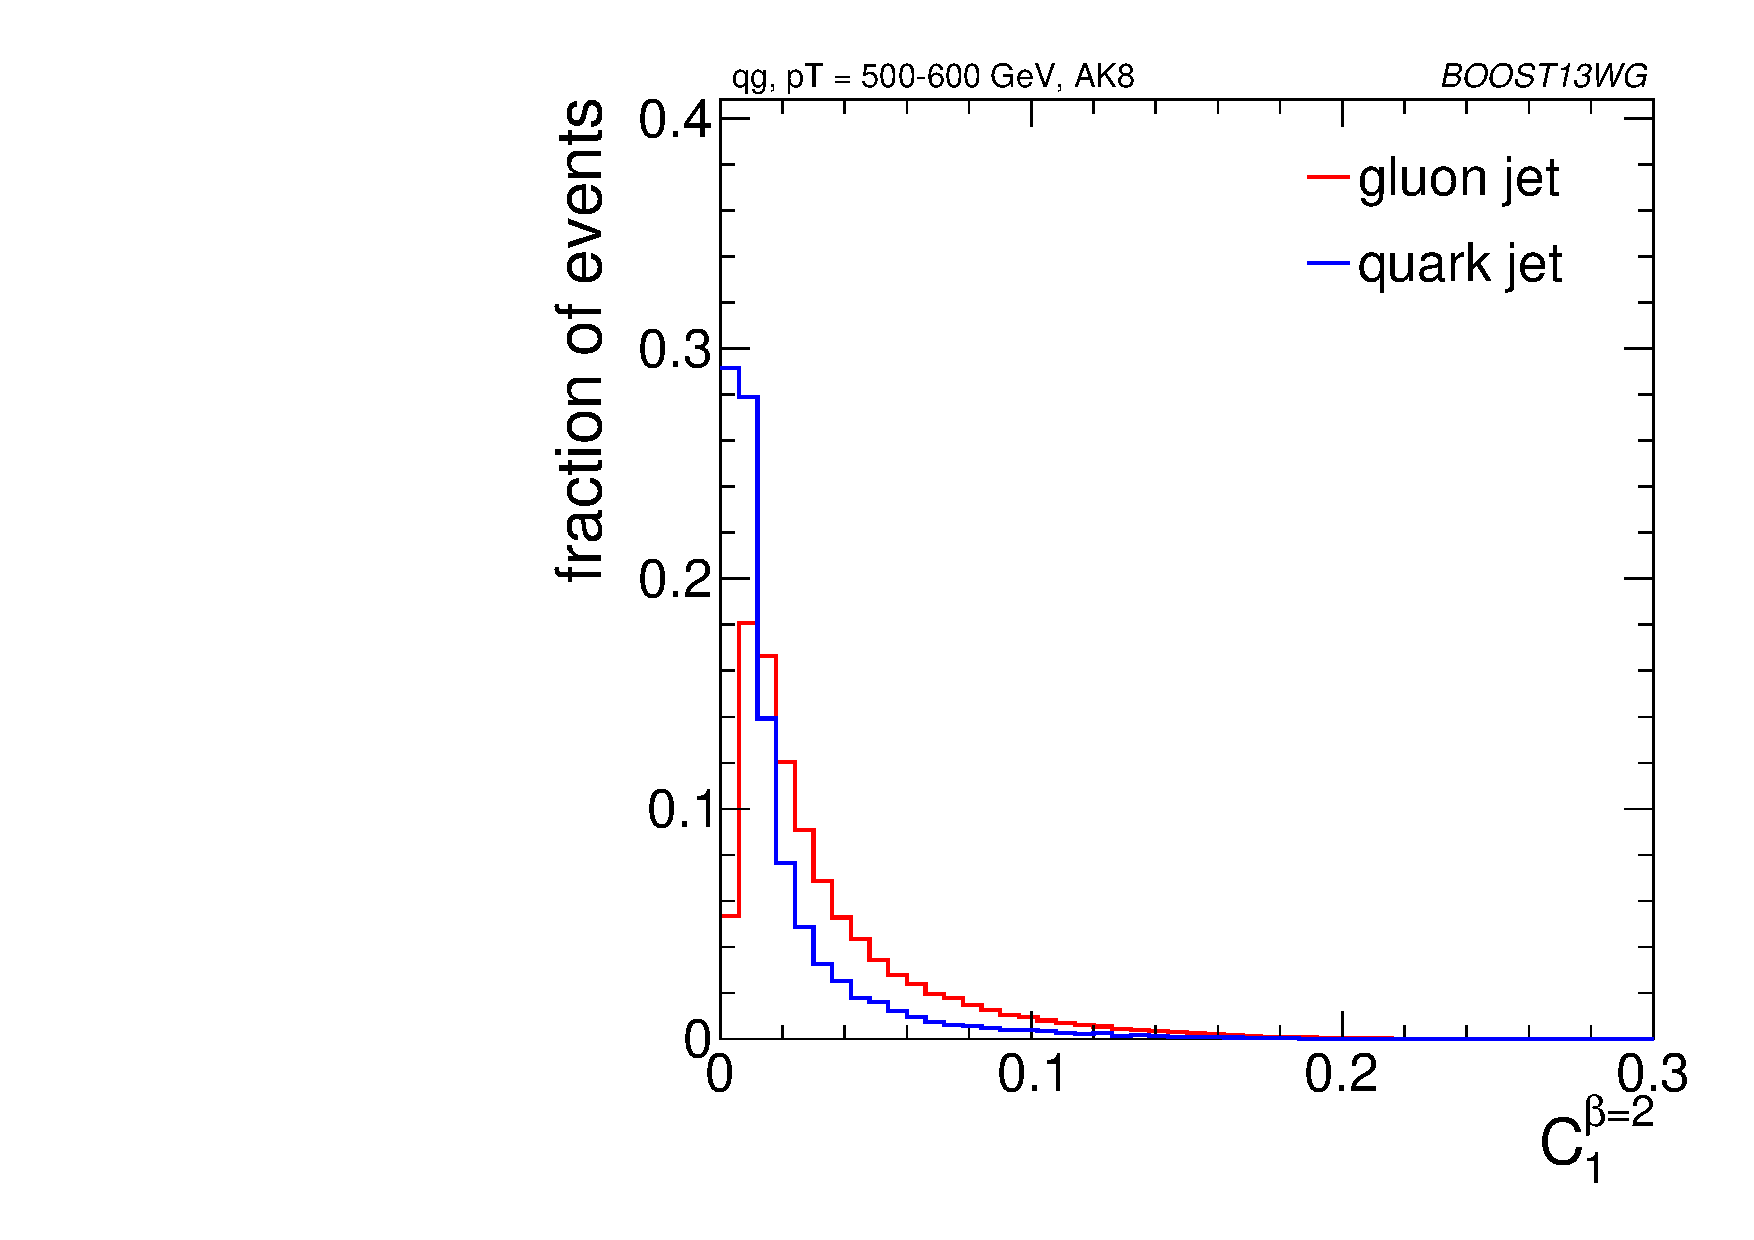
\includegraphics[width=0.30\textwidth]{./Figures/QGTagging/pT500/AKtR08/h_c1_b2.pdf}}
\subfigure[$\tau_{1}^{\beta=2}$]{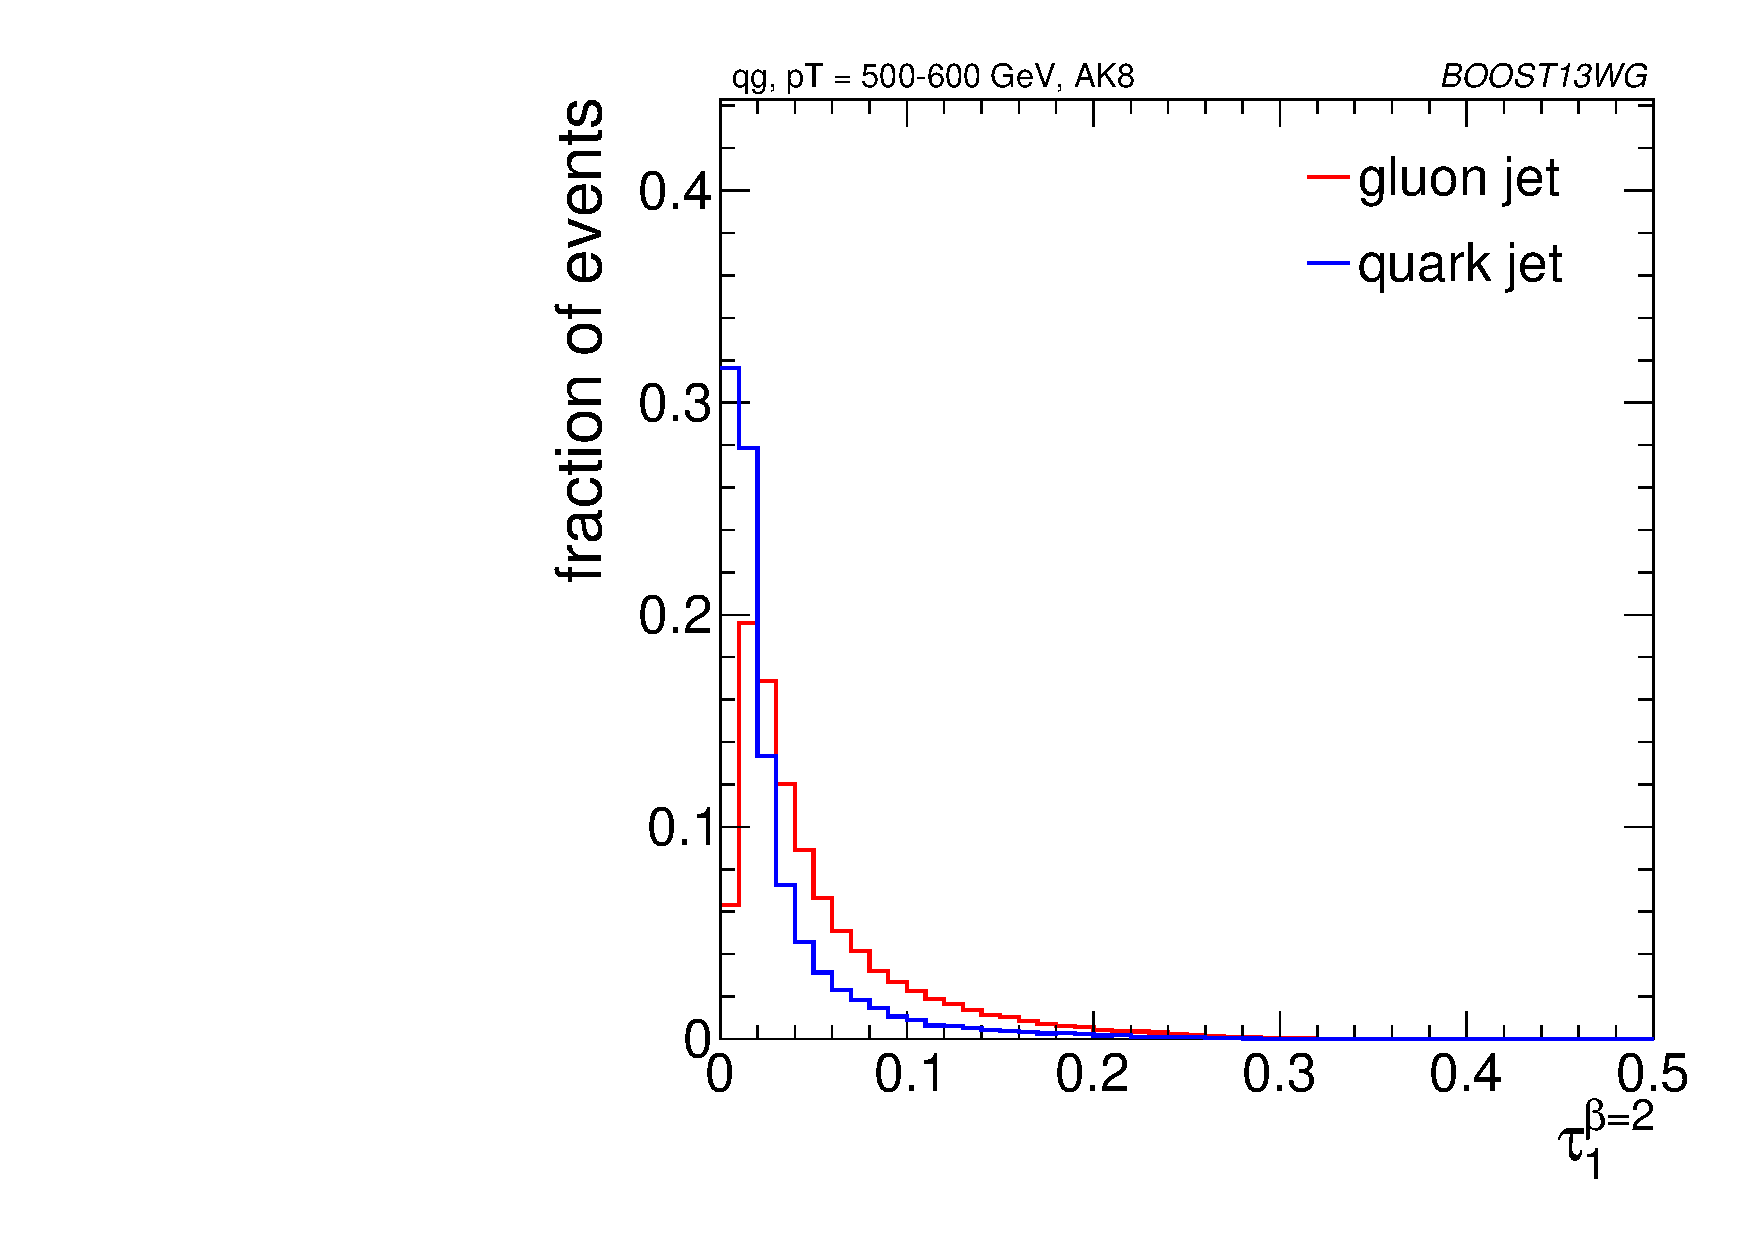
\includegraphics[width=0.30\textwidth]{./Figures/QGTagging/pT500/AKtR08/h_tau1_b2.pdf}}
\subfigure[Ungroomed mass]{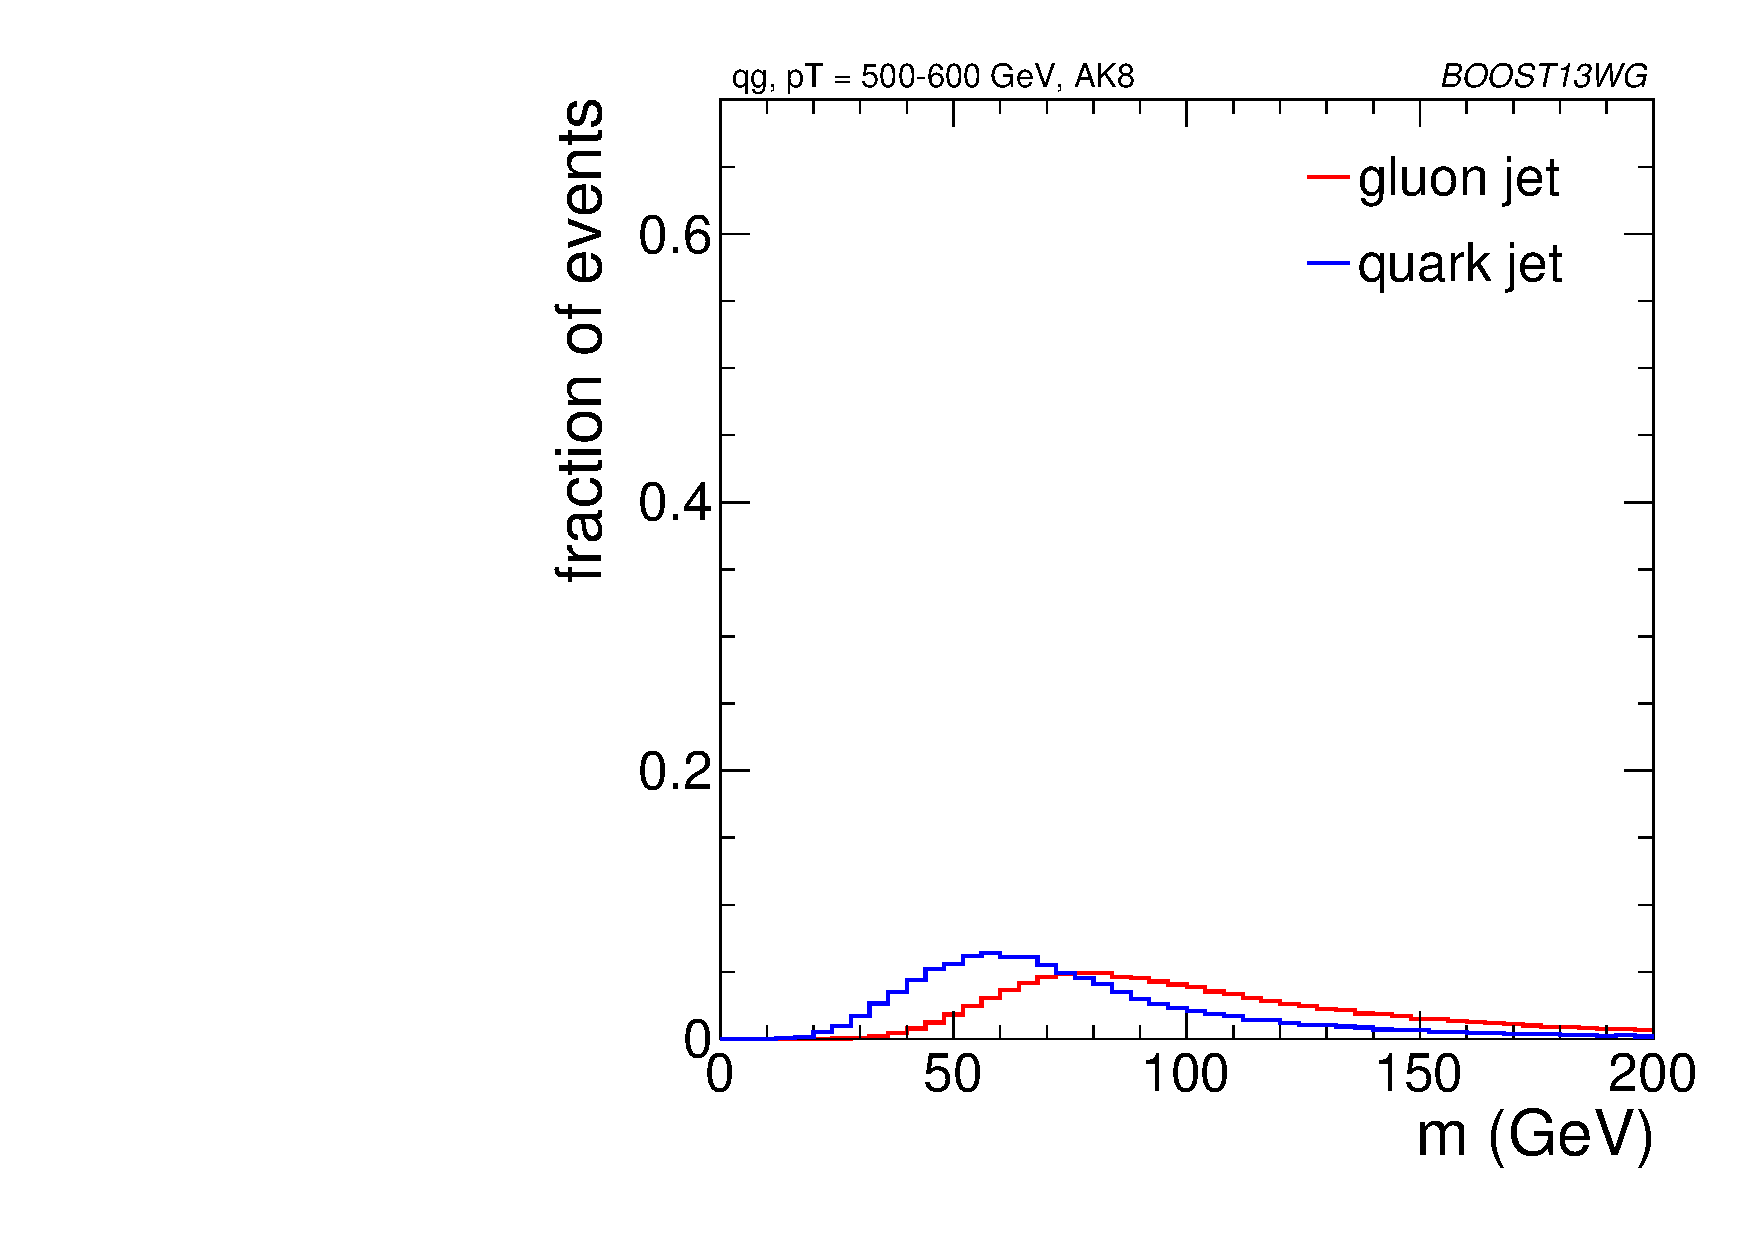
\includegraphics[width=0.30\textwidth]{./Figures/QGTagging/pT500/AKtR08/jmass1.pdf}}
\caption{Comparisons of quark and gluon distributions of different substructure variables, organized by Class, for leading jets in the 
$\pt=500-600 \GeV$ bin using the anti-\kT $R=0.8$ algorithm. The first three plots are Classes I-III, with Class IV in the second row, and Class V in the third row.}
\label{fig:qg_pt500_subst_AKt_R08}
\end{figure*}

%The quark and gluon distributions of different substructure observables
%are shown in Figure~\ref{fig:qg_pt500_subst_AKt_R08} (in the $\pt=500-600\GeV$ bin and $R=0.8$), and these illustrate some of the distinctions between the Classes made above. 
In Figure~\ref{fig:qg_pt500_subst_AKt_R08} are shown the quark and
gluon distributions of different substructure observables in the
$\pt=500-600\GeV$ bin for $R=0.8$ jets. These distributions illustrate some of the distinctions between the Classes made above. 
The fundamental difference between quarks and gluons, namely their color charge and consequent amount of radiation in the jet, is clearly indicated in Figure~\ref{fig:qg_pt500_subst_AKt_R08}(a), 
suggesting that simply counting constituents  provides good separation between quark and gluon jets.  In fact, among the observables
considered, one can see by eye that $n_{\rm constits}$ should provide the highest separation
power, \textit{i.e.}, the quark and gluon distributions are most distinct, as was originally noted in \cite{Gallicchio:2011xq,Gallicchio:2012ez}. 
Figure~\ref{fig:qg_pt500_subst_AKt_R08} further suggests
that $C_1^{\beta=0}$ should provide the next best separation, followed by $C_1^{\beta=1}$, as was also
found by the CMS and ATLAS Collaborations \cite{CMS:2013kfa,Aad:2014gea}.   

To more quantitatively study the power of each observable as a
discriminator for quark/gluon tagging, Receiver Operating Characteristic (ROC) curves are built by scanning each distribution
and plotting the background efficiency (to select gluon jets) vs.~the signal efficiency (to select quark jets). 
Figure~\ref{fig:qg_pt300_single} shows these ROC curves for all of the
substructure variables shown in 
Figure~\ref{fig:qg_pt500_subst_AKt_R08} for $R=0.4, 0.8$ and $1.2$ jets (in the $\pt=300$-$400\GeV$
bin). In addition, the ROC curve for a tagger built from a BDT
combination of all the variables (see Section~\ref{sec:multivariate}) is shown.
%
\begin{figure*}
\centering
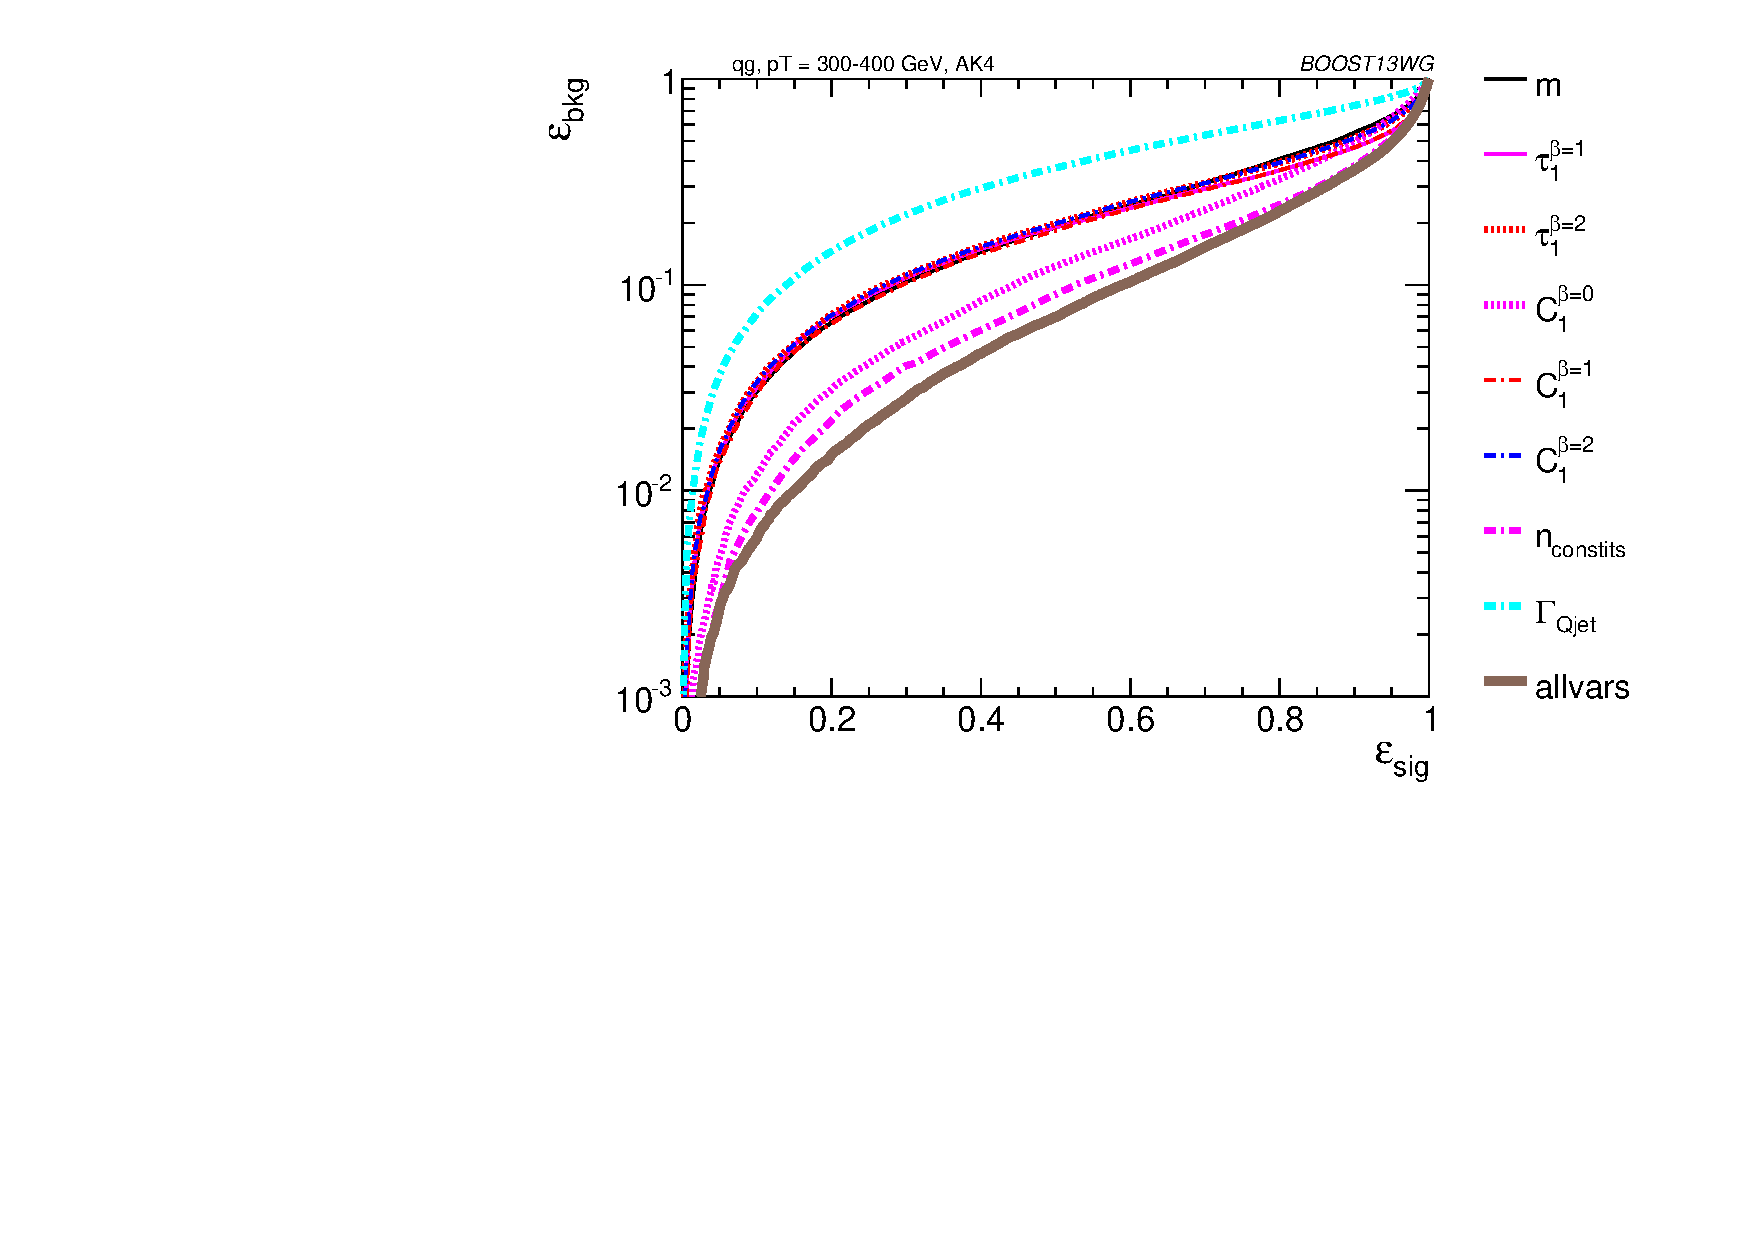
\includegraphics[width=0.48\textwidth]{./Figures/QGTagging/pT300/AKtR04/Rocs_1D_single.pdf}
%\includegraphics[width=0.4\textwidth]{./Figures/QGTagging/pT1000/AKtR04/Rocs_1D_single.pdf}\\
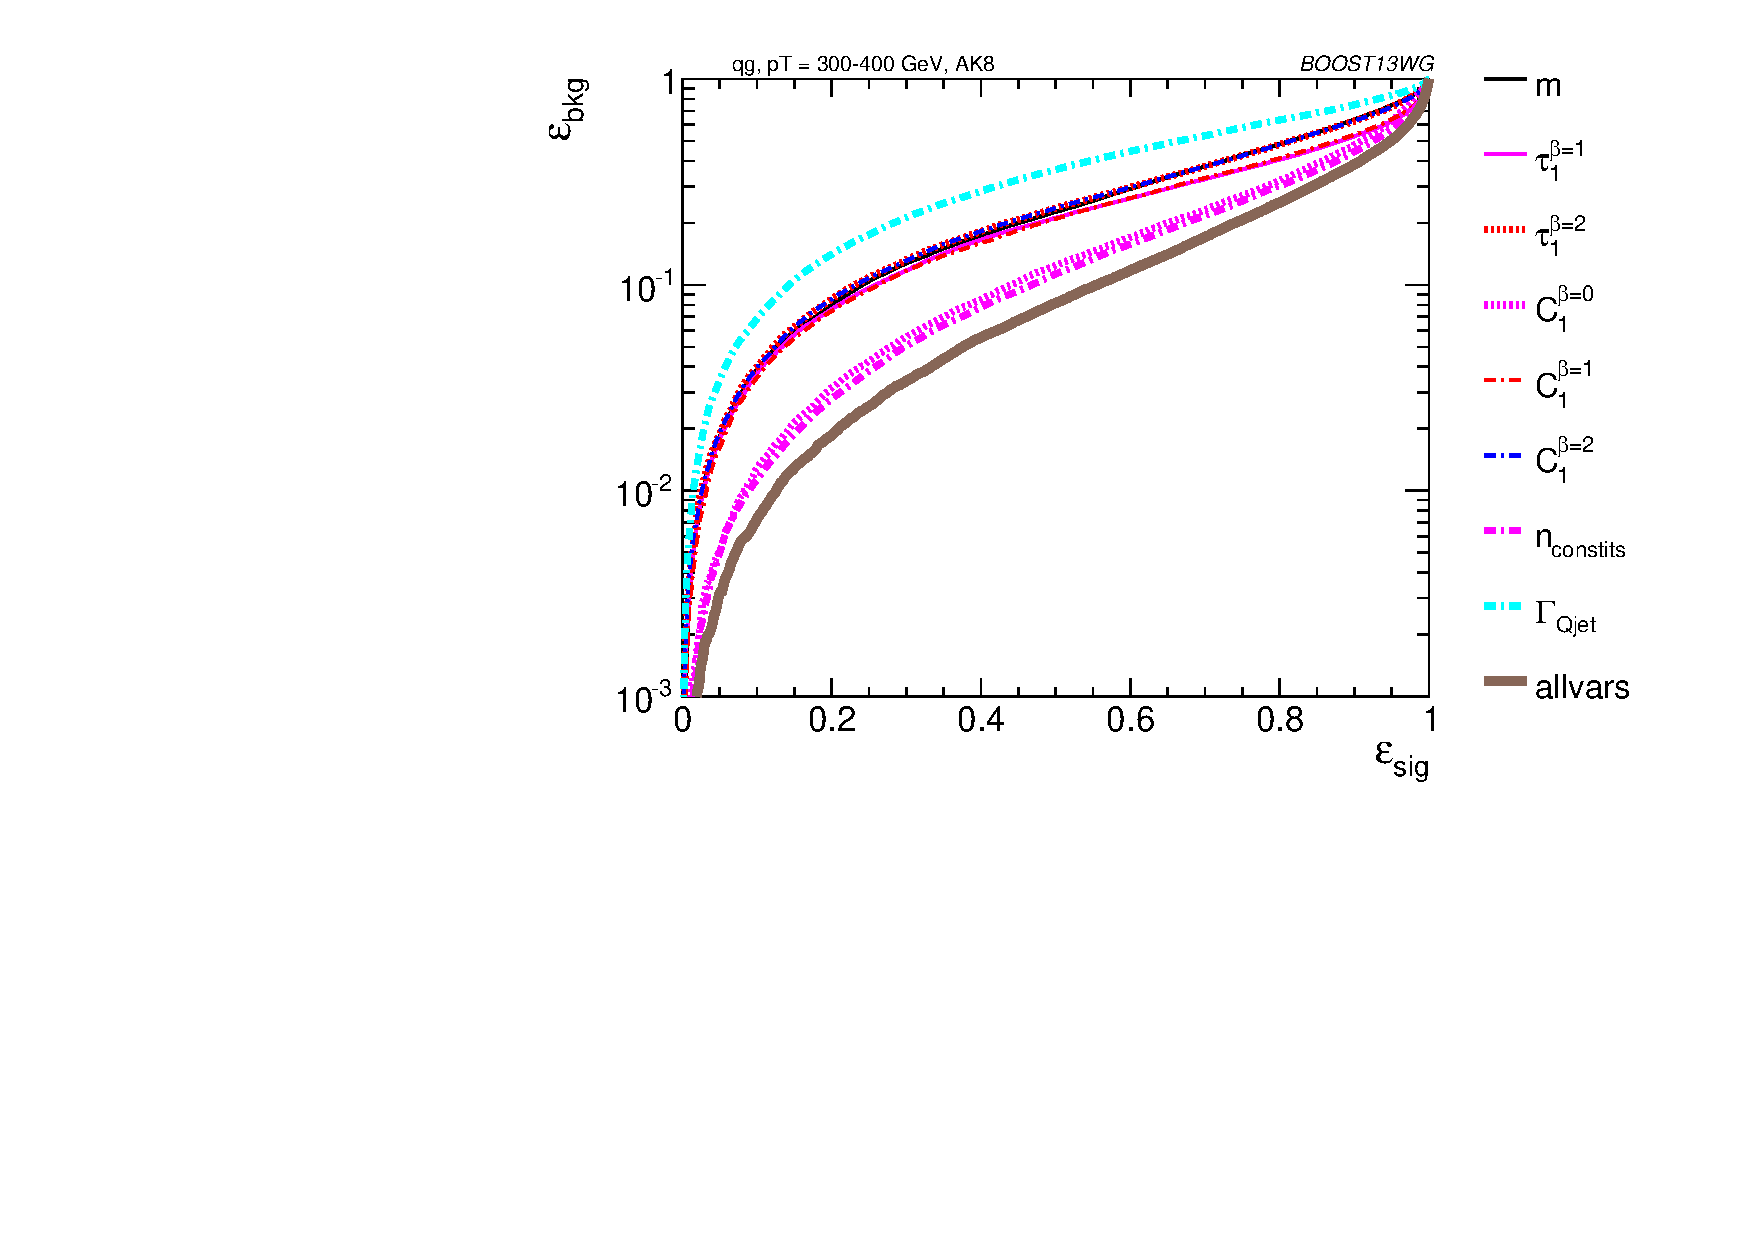
\includegraphics[width=0.48\textwidth]{./Figures/QGTagging/pT300/AKtR08/Rocs_1D_single.pdf}
%\includegraphics[width=0.4\textwidth]{./Figures/QGTagging/pT1000/AKtR08/Rocs_1D_single.pdf}\\
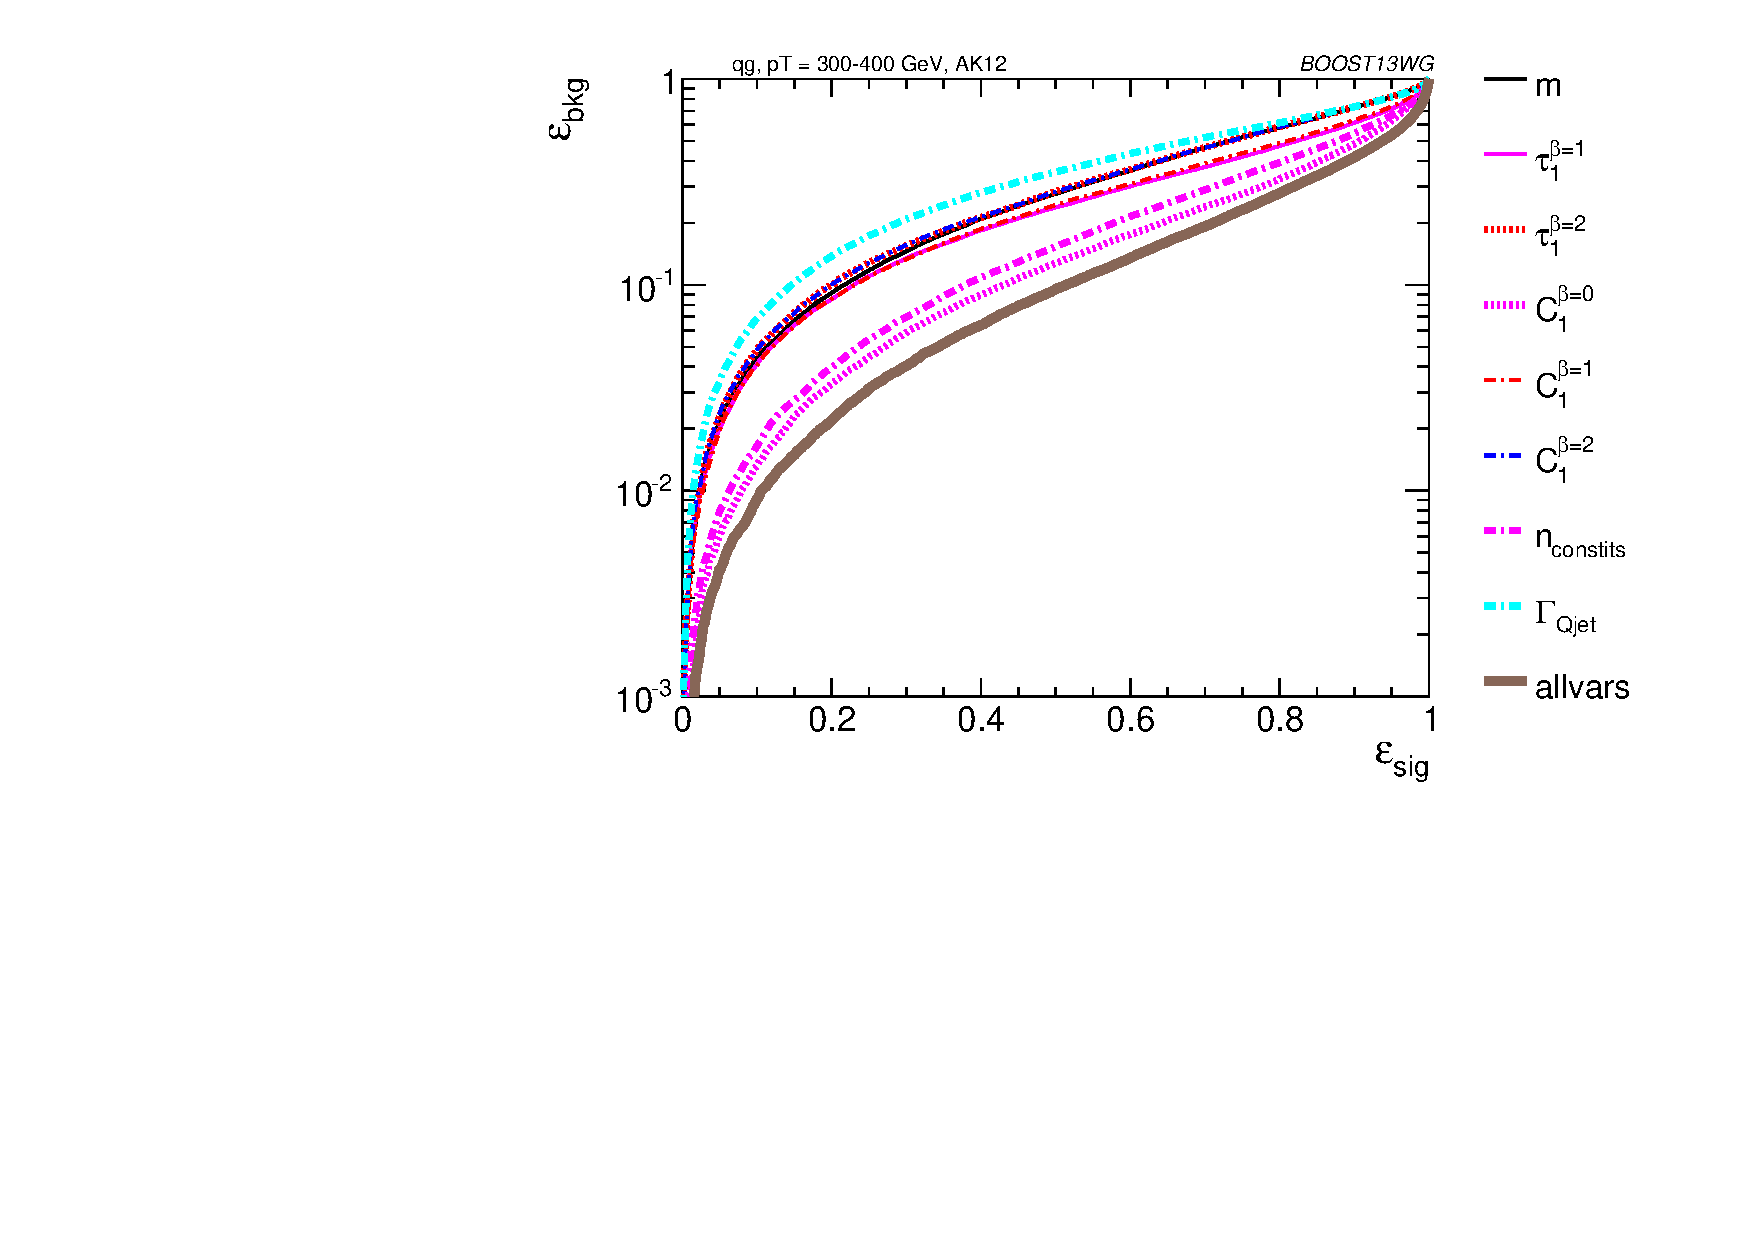
\includegraphics[width=0.48\textwidth]{./Figures/QGTagging/pT300/AKtR12/Rocs_1D_single.pdf}
%\includegraphics[width=0.4\textwidth]{./Figures/QGTagging/pT1000/AKtR12/Rocs_1D_single.pdf}\\
\caption{The ROC curve for all single variables considered for
  quark-gluon discrimination in the \pt 300-400 \GeV bin using the
  \antikt $R=0.4$ (top-left), 0.8 (top-right) and 1.2 (bottom) algorithm.%{\bf ED: Hard to tell the lines on the plots apart}
}
\label{fig:qg_pt300_single}
\end{figure*}
%
As suggested earlier, $n_{\rm constits}$ is the best performing variable for all $R$ values, although $C_1^{\beta=0}$ is not far behind, particularly
for $R=0.8$. Most other variables have similar performance, with the main exception of $\Gamma_{\rm Qjet}$, which shows significantly worse
discrimination (this may be due to our choice of
rigidity $\alpha = 0.1$, with other studies suggesting that a smaller value,
such as $\alpha = 0.01$, produces better results \cite{Ellis:2012sn,Ellis:2014eya}). The combination of all variables shows somewhat better discrimination than any individual observable, and
we  give a more detailed discussion in Section~\ref{sec:qg_combi} of the correlations between the observables and their impact on the combined discrimination power.

%
\begin{figure*}
\centering
\subfigure[$n_ {\rm constits}$]{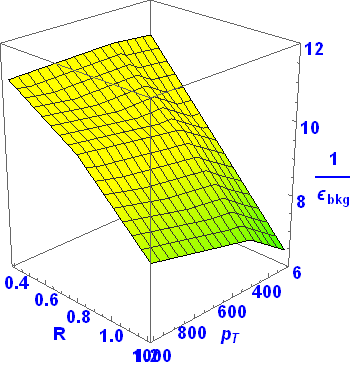
\includegraphics[width=0.30\textwidth]{./Figures/QGSurface/NconB.png}}
\subfigure[$\Gamma_{\rm Qjet}$]{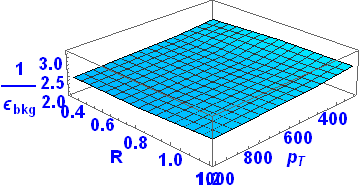
\includegraphics[width=0.30\textwidth]{./Figures/QGSurface/GamQB.png}}
\subfigure[$C_1^{\beta=0}$]{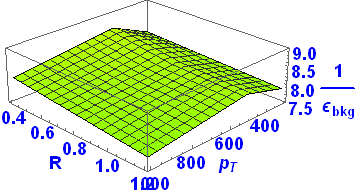
\includegraphics[width=0.30\textwidth]{./Figures/QGSurface/C10B.png}}\\
\subfigure[$C_1^{\beta=1}$]{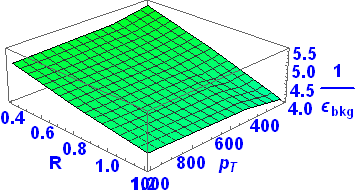
\includegraphics[width=0.30\textwidth]{./Figures/QGSurface/C11B.png}}
\subfigure[$\tau_{1}^{\beta=1}$]{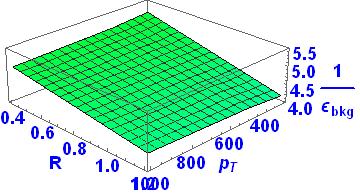
\includegraphics[width=0.30\textwidth]{./Figures/QGSurface/Tau11B.png}}\\
\subfigure[$C_1^{\beta=2}$]{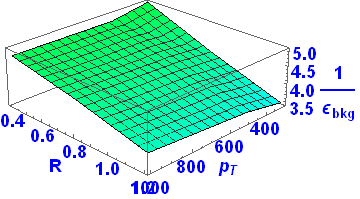
\includegraphics[width=0.30\textwidth]{./Figures/QGSurface/C12B.png}}
\subfigure[$\tau_{1}^{\beta=2}$]{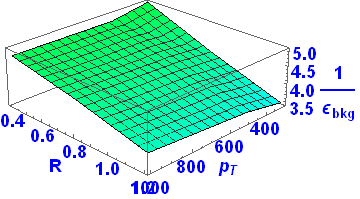
\includegraphics[width=0.30\textwidth]{./Figures/QGSurface/Tau12B.png}}
\subfigure[Ungroomed mass]{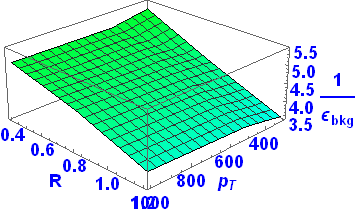
\includegraphics[width=0.30\textwidth]{./Figures/QGSurface/MassB.png}}\\
\caption{Surface plots of $1/\epsilon_\text{bkg}$ for all single variables considered for
  quark-gluon discrimination as functions of $R$ and $\pt$. The first three plots are Classes I-III, with Class IV in the second row, and Class V in the third row. }
\label{fig:qg_surface_single}
\end{figure*}
%

We now examine how the performance of the substructure observables varies with $\pt$ and $R$.  To present the results in a ``digestible'' fashion
we  focus on the gluon jet ``rejection'' factor, $1/\epsilon_\text{bkg}$, for a quark signal efficiency, $\epsilon_\text{sig}$, of $50\,\%$.
We can use the values of $1/\epsilon_\text{bkg}$ generated for the 9 kinematic points introduced above ($R = 0.4, 0.8, 1.2$ and 
the 100 GeV $\pt$ bins with lower limits
$p_T = 300\, \text{GeV}$, $500\, \text{GeV}$, $1000\,\text{GeV}$) to generate surface plots.  The surface plots in Figure~\ref{fig:qg_surface_single}
indicate both the level of gluon rejection
and the variation with $\pt$ and $R$ for each of the studied single observable. 
The color shading in these plots is defined so that a value of $1/\epsilon_\text{bkg}\simeq 1$ yields the color ``violet'', while 
$1/\epsilon_\text{bkg}\simeq 20 $ yields the color ``red''.   The ``rainbow'' of colors in between vary linearly with $\log_{10} (1/\epsilon_\text{bkg})$. 
% The colors have the same correlation with the magnitude of $1/\epsilon_\text{bkg}$
%in all of the plots, but repeat after a change of about 4.  Thus ``blue'' corresponds to a value of about 2.5 in  Figure~\ref{fig:qg_surface_single}(b) and the
%values 6.5 and 10.5
%in  Figure~\ref{fig:qg_surface_single}(a), while ''yellow'' corresponds to about 5 in  Figures~\ref{fig:qg_surface_single}(c) to (h) and about 9 in
% Figure~\ref{fig:qg_surface_single}(a).

 We organize our results by the classes introduced in the previous subsection:

\noindent{\bf Class I:}~The sole constituent of this class is $n_{\rm constits}$. We see in  Figure~\ref{fig:qg_surface_single}(a) that, as expected,  the numerically largest rejection rates occur
for this observable, with the rejection factor ranging from 6 to 11 and 
varying rather dramatically with $R$.  As $R$ increases the jet collects more constituents from the underlying event, which are the same
for quark and gluon jets, and the separation power decreases.  At large $R$, there is some improvement with increasing $\pt$ due to the 
enhanced QCD radiation, which is different for quarks vs.~gluons.  

\noindent{\bf Class II:}~The variable $\Gamma_{\rm Qjet}$ constitutes this class. Figure~\ref{fig:qg_surface_single}(b) confirms the limited efficacy of this single
observable (at least for our parameter choices) with a rejection rate only in the range 2.5 to 2.8.  On the other hand, this 
observable probes a very different
property of jet substructure, \textit{i.e.}, the sensitivity to detailed changes in the grooming procedure, and this difference is suggested
by the distinct $R$ and $\pt$ dependence illustrated in  Figure~\ref{fig:qg_surface_single}(b).  The rejection rate increases with increasing $R$
and decreasing $\pt$, since the distinction between quark and gluon jets for this observable arises from the relative importance of the one
``hard'' gluon emission configuration.  The role of this contribution is enhanced for both decreasing $\pt$ and increasing $R$. 


\noindent{\bf Class III:}~The only member of this class is $C_1^{\beta=0}$. Figure~\ref{fig:qg_surface_single}(c) indicates that this observable  can itself provide a rejection rate in the range
7.8 to 8.6 (intermediate between the two previous observables), and again with distinct $R$ and $\pt$ dependence.  In this case the rejection
rate decreases slowly with increasing $R$, which follows from the fact that $\beta = 0$ implies no weighting of $\Delta R$ in the definition of $C_1^{\beta=0}$, greatly reducing 
the angular dependence.
The rejection rate peaks at intermediate $\pt$ values, an effect visually enhanced by the limited number of 
$\pt$ values included.  

%Both the distinct values of the rejection rates and the differing $R$ and $\pt$ dependence serve to confirm that these three
%observables tend to probe independent features of the quark and gluon jets.  

\noindent{\bf Class IV:}~Figures~\ref{fig:qg_surface_single}(d) and (e)  confirm
the very similar properties of the observables $C_1^{\beta=1}$ and $\tau_1^{\beta=1}$ (as already suggested in
Figures~\ref{fig:qg_pt500_subst_AKt_R08}(d) and (e)). They have
 essentially identical rejection rates (4.1 to 5.4) and identical $R$ and $\pt$ dependence (a slow decrease with increasing $R$ and an even
slower increase with increasing $\pt$).  

\noindent{\bf Class V}:~The observables $C_1^{\beta=2}$, $\tau_1^{\beta=2}$, and $m$ have similar rejection rates in the 
range 3.5 to 5.3, as well as very similar $R$ and $\pt$ dependence (a slow decrease with increasing $R$ and an even
slower increase with increasing $\pt$).  

Arguably, drawing a distinction between the Class IV and Class V observables is a fine point, 
but the color shading does suggest some
distinction from the slightly smaller rejection rate in Class V.  Again the strong similarities between the plots within the second and third rows in 
Figure~\ref{fig:qg_surface_single} speaks to the common properties of the observables within the two classes.


 
%For jet masses, few variations are observed as the 
%radius parameter of the jet reconstruction is increased in the two highest $\pt$ bins; this is because the radiation
%is more collimated and the dependence on $R$ is consequently smaller.
%However, for the $300-400\GeV$ bin, the use of small-$R$ jets produces a shift in the
%mass distributions towards lower values, so that large-$R$ jet masses are more stable
%with $\pt$ and small-$R$ jet masses are smaller at low-$\pt$ as expected from the spatial
%constraints imposed by the $R$ parameter. These statements are explored more 
%quantitatively later in this section. ({\bf BS: Do we have plots for this?})

%The evolution of some of the substructure variable distributions with $\pt$ and R is less trivial than
%for the jet masses. In particular, changing the $R$ parameter at high $\pt$ changes significantly the $C_a^{\beta}$
%for $\beta>0$ and the $n_{\rm constits}$ distributions, while leaving all other distributions qualitatively unchanged. 
%This is illustrated in Figure~\ref{fig:Rdep_qg_C_pt1000} for $\beta=0$ and $\beta=1$ using $a=1$ in both cases for
%jets with $\pt=1.0-1.1\TeV$. 

 %
%\begin{figure*}
%\centering
%\subfigure[$C_1^{\beta=0}$, $R=0.4$]{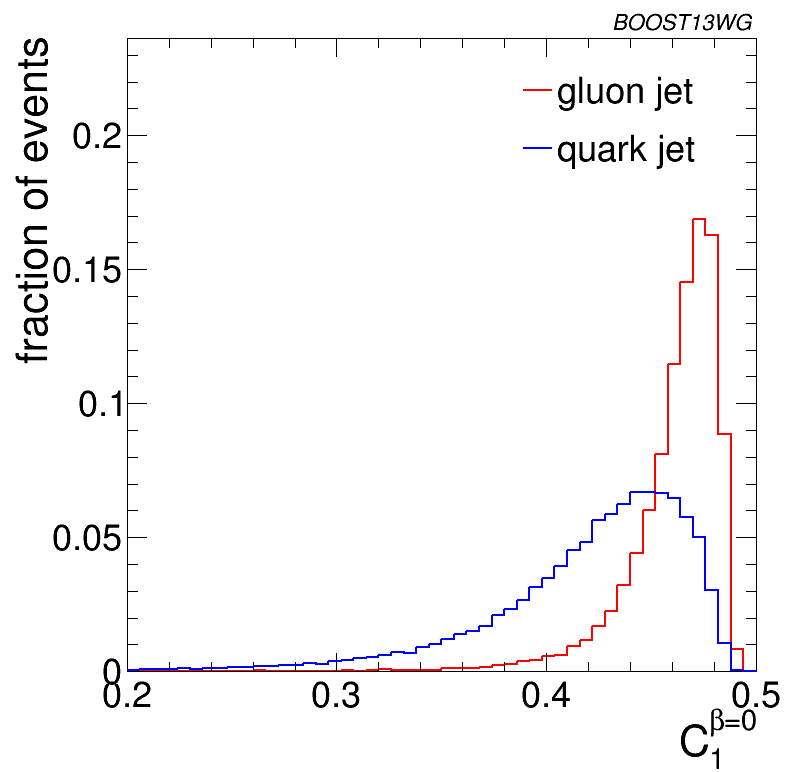
\includegraphics[width=0.30\textwidth]{./Figures/QGTagging/pT1000/AKtR04/h_c1_b0.png}}
%\subfigure[$C_1^{\beta=0}$, $R=0.8$]{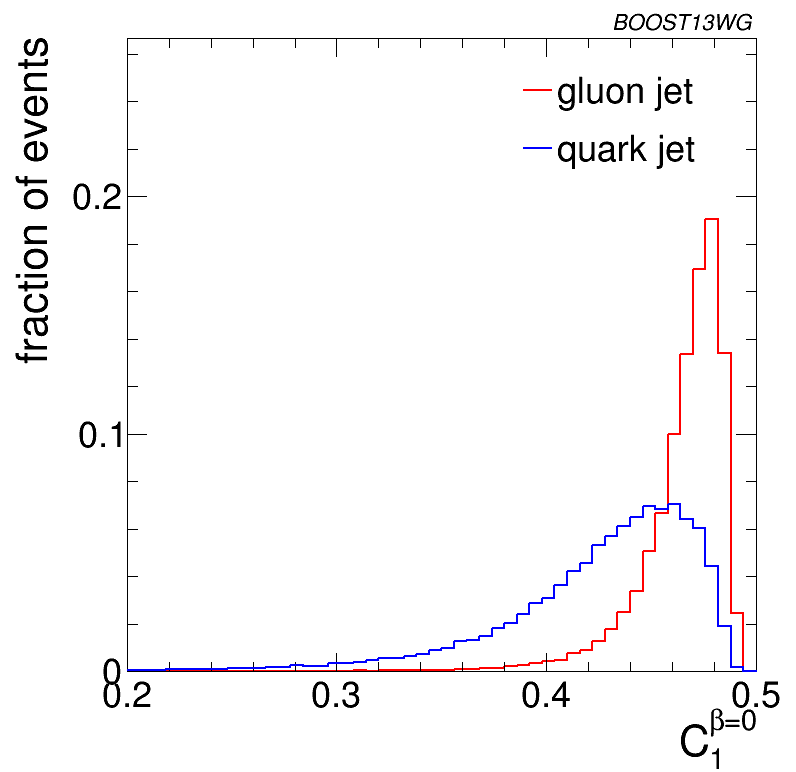
\includegraphics[width=0.30\textwidth]{./Figures/QGTagging/pT1000/AKtR08/h_c1_b0.png}}
%\subfigure[$C_1^{\beta=0}$, $R=1.2$]{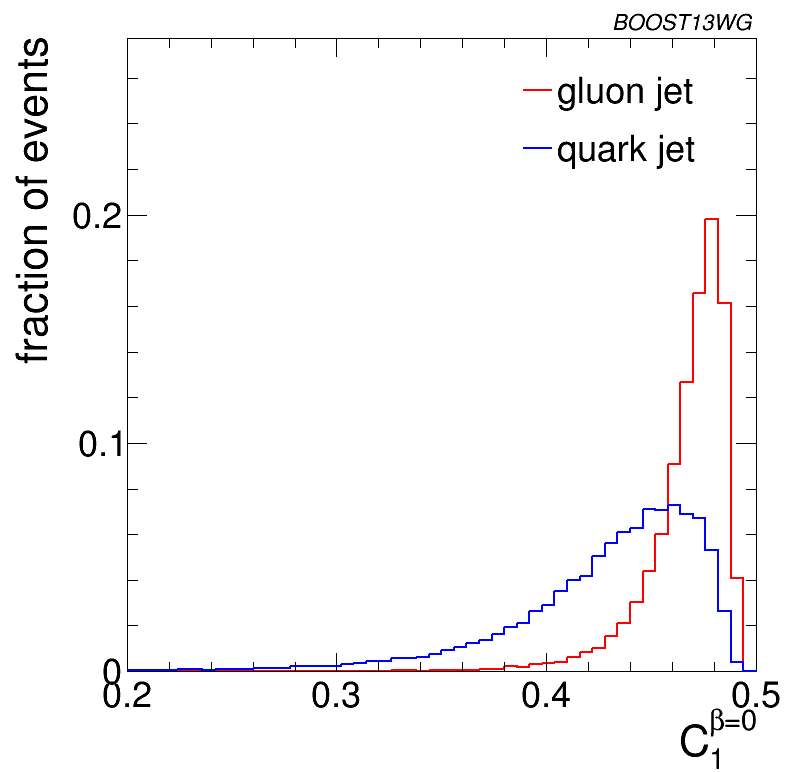
\includegraphics[width=0.30\textwidth]{./Figures/QGTagging/pT1000/AKtR12/h_c1_b0.png}}\\
%\subfigure[$C_1^{\beta=1}$, $R=0.4$]{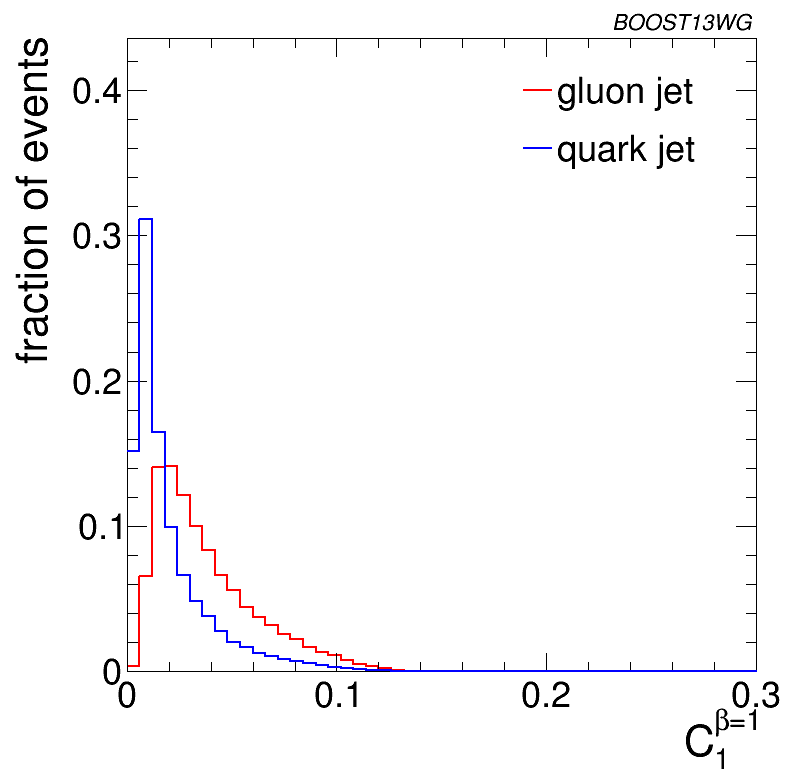
\includegraphics[width=0.30\textwidth]{./Figures/QGTagging/pT1000/AKtR04/h_c1_b1.png}}
%\subfigure[$C_1^{\beta=1}$, $R=0.8$]{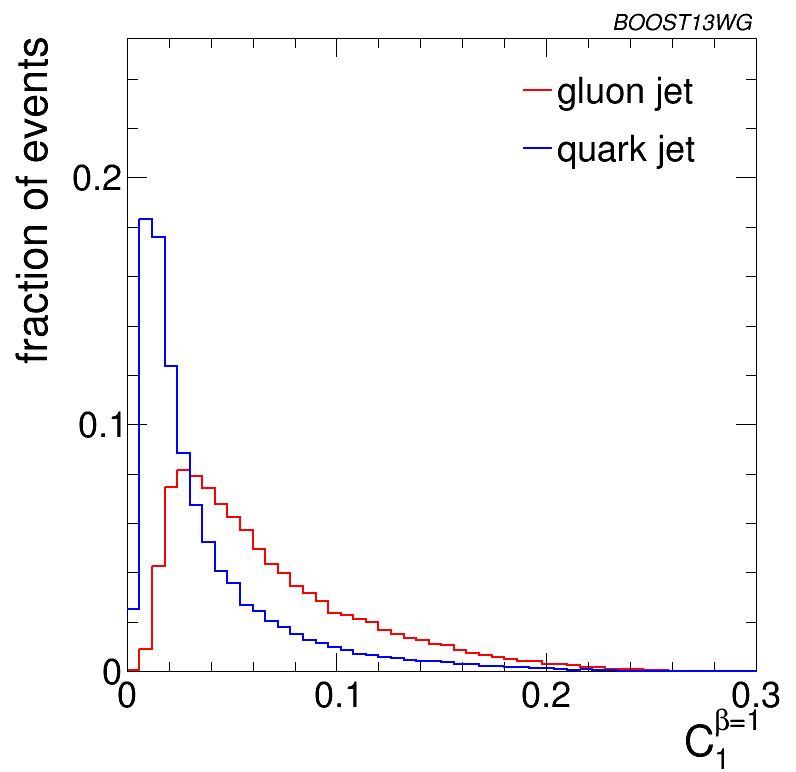
\includegraphics[width=0.30\textwidth]{./Figures/QGTagging/pT1000/AKtR08/h_c1_b1.png}}
%\subfigure[$C_1^{\beta=1}$, $R=1.2$]{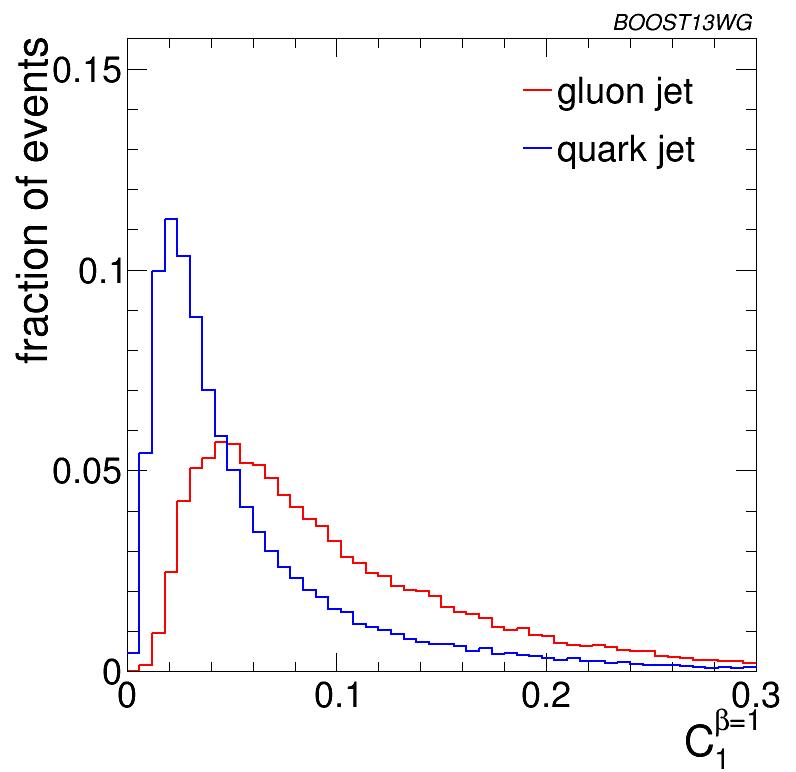
\includegraphics[width=0.30\textwidth]{./Figures/QGTagging/pT1000/AKtR12/h_c1_b1.png}}\\
%\caption{Comparisons of quark and gluon distributions of $C_1^{\beta=0}$ (top) and $C_1^{\beta=1}$ (bottom) 
%for leading jets in the $\pt=1-1.1 \TeV$ bin using the anti-\kT algorithm with $R=0.4$, 0.8 and 1.2. }
%\label{fig:Rdep_qg_C_pt1000}
%\end{figure*}
%The shift towards lower values with changing R is evident for the $C_1^{\beta=1}$ distributions, while the stability
%of $C_1^{\beta=0}$ can also be observed. These features are present in all $\pt$ bins studied, but are even more
%pronounced for lower $\pt$ bins. The shape of the Q-jet volatility distribution shows some non-trivial shape that
%deserves some explanation. Two peaks are observed, one at low volatility values and one at mid-volatility. These
%peaks are generated by two somewhat distinct populations. The high volatility peak arises from jets that get their
%mass primarily from soft (and sometimes wide-angle) emissions. The removal of some of the constituents when
%building Q-jets thus changes the mass significantly, increasing the volatility. The lower volatility peak corresponds
%to jets for which mass is generated by a hard emission, which makes the fraction of Q-jets that change 
%the mass significantly to be smaller. Since the probability of a hard emission is proportional to the colour
%charge (squared),  the volatility peak is higher for gluon jets by about the colour factor $C_A/C_F$. 



In summary, the overall discriminating power between quark and gluon jets tends to
 decrease with increasing $R$, except for the $\Gamma_{\rm Qjet}$ observable, presumably in large part due to the
 contamination from the underlying event. Since the construction of the $\Gamma_{\rm Qjet}$ observable explicitly
involves pruning away the soft, large angle constituents, it is not surprising that it exhibits different $R$ dependence. 
In general the discriminating power increases slowly and monotonically
with $\pt$ (except for the $\Gamma_{\rm Qjet}$ and $C_1^{\beta=0}$ observables). This is presumably due to the overall
increase in radiation from high $\pt$ objects, which accentuates the differences in the quark and gluon color charges and 
 providing some increase in discrimination.  
In the following section, we study the effect of combining multiple observables.

%
\begin{figure*}
\centering
\subfigure[$C_1^{\beta=1}+\tau_{1}^{\beta=1}$]{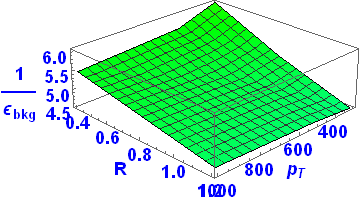
\includegraphics[width=0.30\textwidth]{./Figures/QGSurface/C11Tau11B.png}}
\subfigure[$C_1^{\beta=2}+\tau_{1}^{\beta=2}$]{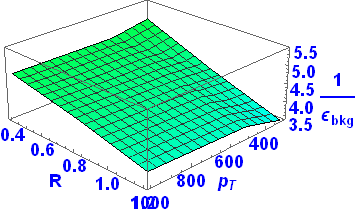
\includegraphics[width=0.30\textwidth]{./Figures/QGSurface/C12Tau12B.png}}
%\subfigure[$C_1^{\beta=0}$]{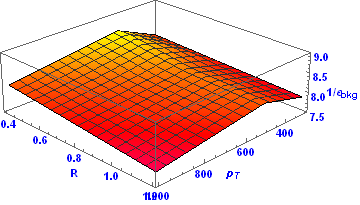
\includegraphics[width=0.30\textwidth]{./Figures/QGSurface/C10.png}}\\
%\subfigure[$C_1^{\beta=1}$]{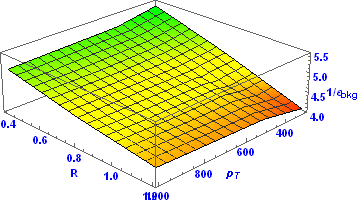
\includegraphics[width=0.30\textwidth]{./Figures/QGSurface/C11.png}}
%\subfigure[$\tau_{1}^{\beta=1}$]{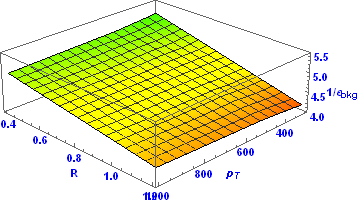
\includegraphics[width=0.30\textwidth]{./Figures/QGSurface/Tau11.png}}\\
%\subfigure[$C_1^{\beta=2}$]{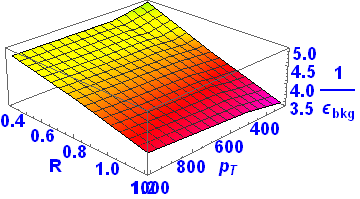
\includegraphics[width=0.30\textwidth]{./Figures/QGSurface/C12.png}}
%\subfigure[$\tau_{1}^{\beta=2}$]{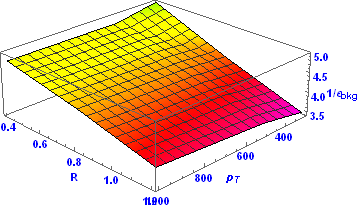
\includegraphics[width=0.30\textwidth]{./Figures/QGSurface/Tau12.png}}
%\subfigure[Ungroomed mass]{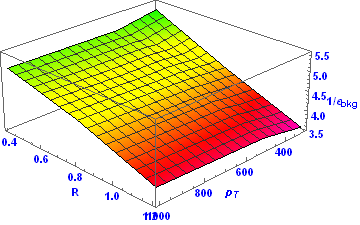
\includegraphics[width=0.30\textwidth]{./Figures/QGSurface/Mass.png}}\\
\caption{Surface plots of $1/\epsilon_\text{bkg}$ for the indicated pairs of variables from (a) Class IV and (b) Class V considered for
  quark-gluon discrimination as functions of $R$ and $\pt$. }
\label{fig:qg_surface_pairA}
\end{figure*}
%


\subsection{Combined Performance and Correlations}\label{sec:qg_combi}
Combining multiple observables in a BDT can give further improvement over cuts on a single variable. Since the improvement from combining correlated observables is expected to be inferior to that from combining uncorrelated observables, studying the performance of multivariable combinations gives insight into the correlations between substructure variables and the physical  
features allowing for quark/gluon discrimination. Based on our discussion of the correlated properties
of observables within a single class, we expect little improvement in the rejection rate when combining observables from the same class,
and substantial improvement when combining observables from different classes.  Our classification of observables for quark/gluon tagging  therefore motivates the study of
particular combinations of variables for use in experimental analyses.
 
 To quantitatively study the improvement obtained from multivariate analyses, we build quark/gluon taggers from
every pair-wise combination of variables studied in the previous section; we also compare the pair-wise performance with the all-variables combination.
  To illustrate the results achieved in this way, we use the same  2D 
surface plots as in Figure~\ref{fig:qg_surface_single}.  
Figure~\ref{fig:qg_surface_pairA} shows pair-wise plots for variables in (a) Class IV and (b) Class V, respectively.  Comparing to the corresponding plots
in Figure~\ref{fig:qg_surface_single}, we see that combining $C_1^{\beta=1}+\tau_{1}^{\beta=1}$ provides a 
small ($\sim10\%$) improvement in the rejection rate  with essentially no change in the $R$ and $\pt$ dependence, while combining $C_1^{\beta=2}+\tau_{1}^{\beta=2}$   
yields a rejection rate that is essentially identical to the single observable rejection rate for all $R$ and $\pt$ values (with a similar conclusion if one
of these observables is replaced with the ungroomed jet mass $m$).  
This  confirms the expectation that the
observables within a single class effectively probe the \textit{same} jet properties.

 
%
\begin{figure*}
\centering
\subfigure[$n_{\rm constits}+\Gamma_{\rm Qjet}$]{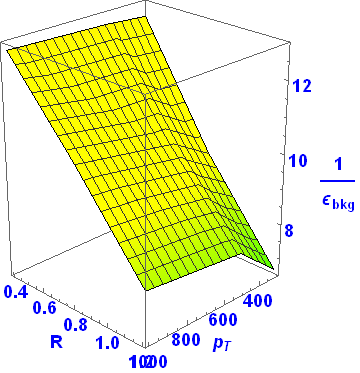
\includegraphics[width=0.28\textwidth]{./Figures/QGSurface/NconGamQB.png}}
\subfigure[$n_{\rm constits}+ C_1^{\beta=1}$]{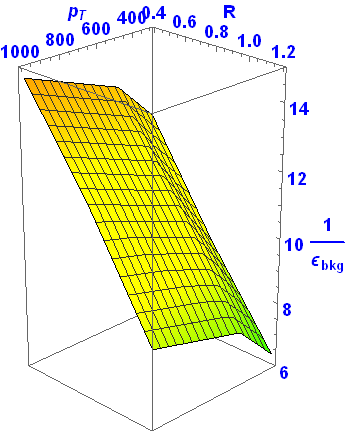
\includegraphics[width=0.28\textwidth]{./Figures/QGSurface/NconC11B.png}}
\subfigure[$n_{\rm constits}+ C_1^{\beta=2}$]{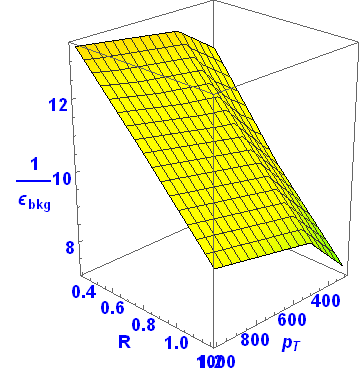
\includegraphics[width=0.28\textwidth]{./Figures/QGSurface/NconC12B.png}}\\
\subfigure[$n_{\rm constits}+ C_1^{\beta=0}$]{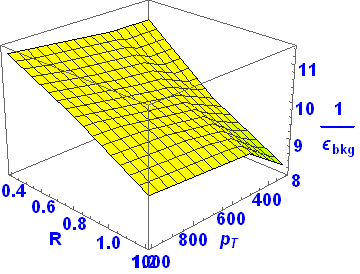
\includegraphics[width=0.28\textwidth]{./Figures/QGSurface/NconC10B.png}}
\subfigure[$n_{\rm constits}+ \tau_1^{\beta=1}$]{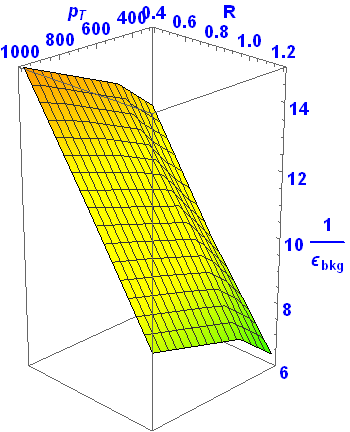
\includegraphics[width=0.28\textwidth]{./Figures/QGSurface/NconTau11B.png}}
\subfigure[$\Gamma_{\rm Qjet}+ C_{1}^{\beta=0}$]{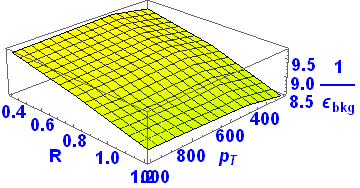
\includegraphics[width=0.28\textwidth]{./Figures/QGSurface/C10GamQB.png}}\\
\subfigure[$\Gamma_{\rm Qjet}+ C_{1}^{\beta=1}$]{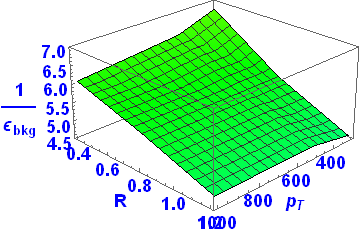
\includegraphics[width=0.28\textwidth]{./Figures/QGSurface/C11GamQB.png}}
\subfigure[$\Gamma_{\rm Qjet}+ C_{1}^{\beta=2}$]{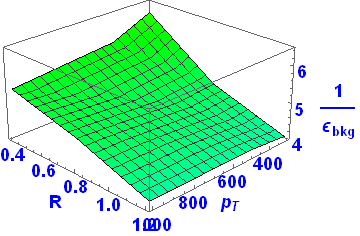
\includegraphics[width=0.28\textwidth]{./Figures/QGSurface/C12GamQB.png}}
\subfigure[$ C_{1}^{\beta=0}+ C_{1}^{\beta=1}$]{\includegraphics[width=0.28\textwidth]{./Figures/QGSurface/C10C11B.png}}\\
\subfigure[$ C_{1}^{\beta=0}+ C_{1}^{\beta=2}$]{\includegraphics[width=0.28\textwidth]{./Figures/QGSurface/C10C12B.png}}
\subfigure[$ C_{1}^{\beta=1}+ C_{1}^{\beta=2}$]{\includegraphics[width=0.28\textwidth]{./Figures/QGSurface/C11C12B.png}}
\subfigure[All]{\includegraphics[width=0.28\textwidth]{./Figures/QGSurface/AllB.png}}
\caption{Surface plots of $1/\epsilon_\text{bkg}$ for the indicated pairs of variables from different classes considered for
  quark-gluon discrimination as functions of $R$ and $\pt$. }
\label{fig:qg_surface_pairB}
\end{figure*}
%

Next, we consider  cross-class pairs of observables  in Figure~\ref{fig:qg_surface_pairB}, where, except in the one case noted below,
we use only a single observable from each class for illustrative purposes.
Since $n_{\rm constits}$ is the best performing single variable, the largest rejection
rates are obtained from combining another observable with $n_ {\rm constits}$ (Figures~\ref{fig:qg_surface_pairB}(a) to (e)).  
In general, the rejection rates are larger for the pair-wise case
than for the single variable case.  In particular, the pair $n_{\rm constits}+ C_1^{\beta=1}$ in Figure~\ref{fig:qg_surface_pairB}(b)
yields rejection rates in the range 6.4 to 14.7 with the largest
values at small $R$ and large $\pt$.  As expected, the pair  $n_{\rm constits}+ \tau_1^{\beta=1}$ in Figure~\ref{fig:qg_surface_pairB}(e)
yields very similar rejection rates (6.4 to 15.0), since $C_1^{\beta=1}$ and $\tau_1^{\beta=1}$ are both in Class IV. 
The other pairings with $n_{\rm constits}$ yield smaller 
rejection rates and smaller dynamic ranges.  The pair $n_ {\rm constits}+ C_1^{\beta=0}$ (Figure~\ref{fig:qg_surface_pairB}(d)) exhibits
the smallest range of rates (8.3 to 11.3), suggesting that the differences between these two observables serve to substantially 
reduce the $R$ and $\pt$ dependence for the pair, but this also to reduce the possible optimization.  The other pairs shown exhibit
similar behavior.  

The $R$ and $\pt$ dependence of the pair-wise combinations is generally similar to the single observable with the most dependence 
on $R$ and $\pt$.  The smallest $R$ and $\pt$ variation always occurs 
when pairing with $C_1^{\beta=0}$.  Changing any of the observables in these pairs with a different observable in the same class (\textit{e.g.},
$C_1^{\beta=2}$ for $\tau_1^{\beta=2}$) produces very similar results.  Figure~\ref{fig:qg_surface_pairB}(k) shows the
result of a BDT analysis including all of the current observables with rejection rates in the range 10.5 to 17.1.  This is a somewhat narrower range
than in Figure~\ref{fig:qg_surface_pairB}(b) but with  larger maximum values.

Some features are more easily seen with an alternative presentation of the data:~we fix  $R$ and $\pt$ and simultaneously show the single- and pair-wise  observables performance in a single matrix, and these matrices are shown in Figures~\ref{fig:qg_pt1000_comb} and \ref{fig:qg_akt4_comb}.  
The numbers in each cell are the same rejection rate for gluons used earlier,
 $1/\epsilon_\text{bkg}$, with $\epsilon_\text{sig}= 50\,\% $ (quarks).  Figure~\ref{fig:qg_pt1000_comb} shows the results for $\pt=1-1.1 \TeV$ and
$R =0.4,0.8,1.2$, while  Figure~\ref{fig:qg_akt4_comb} is for $R = 0.4$ and the 3 $\pt$ bins.  The single observable rejection rates appear on the 
diagonal, and the pairwise results are off the diagonal.  The largest pair-wise rejection rate, as already suggested by Figure~\ref{fig:qg_surface_pairB}(e),
appears at large $\pt$ and small $R$ for the pair $n_ {\rm constits}+ \tau_1^{\beta=1}$ 
(with very similar results for $n_ {\rm constits}+ C_1^{\beta=1}$). 
The correlations indicated by the shading\footnote{The connection between the value of the rejection rate and the shading color in 
Figures~\ref{fig:qg_pt1000_comb} and \ref{fig:qg_akt4_comb} is the same as that in Figures~\ref{fig:qg_surface_single} to \ref{fig:qg_surface_pairB}.}   
should be largely understood as indicating the organization of the observables into the now-familiar
classes.  The all-observable (BDT) result appears as the number at the lower right in each plot.

%In order to quantitatively study the value of each variable for quark/gluon tagging, we study the gluon 
%rejection, defined as $1/\epsilon_{\rm gluon}$, at a fixed quark selection efficiency
%of 50\% using jets with $\pt=1-1.1 \TeV$ and for different $R$ parameters. Figure~\ref{fig:qg_pt1000_comb} shows the gluon 
%rejection for each pair-wise combination. 
%The pair-wise gluon rejection at 50\% quark efficiency can be compared to the single-variable
%values shown along the diagonal. The gluon rejection for the 
%BDT all-variable combination is also shown on the bottom right of each plot.

%
\begin{figure*}
\centering
\includegraphics[width=0.48\textwidth]{./Figures/QGTagging/pT1000/AKtR04/effBkg2D.pdf}
\includegraphics[width=0.48\textwidth]{./Figures/QGTagging/pT1000/AKtR08/effBkg2D.pdf}
\includegraphics[width=0.48\textwidth]{./Figures/QGTagging/pT1000/AKtR12/effBkg2D.pdf}
\caption{Gluon rejection defined as $1/\epsilon_{\rm gluon}$ when using each 2-variable combination 
as a tagger with 50\% acceptance for quark jets. Results are shown for
jets with $\pt=1-1.1 \TeV$ and
for (top left) $R=0.4$; (top right) $R=0.8$; (bottom) $R=1.2$. The rejection obtained with a tagger that uses all variables is also shown
in the plots. }
\label{fig:qg_pt1000_comb}
\end{figure*}
%

%As already observed in the previous section, $n_{\rm constits}$ is the most powerful single variable and
%$\C{1}{\beta=0}$ follows closely. However, the gains are largely correlated; the combined performance of $n_{\rm constits}$ and $\C{1}{\beta=0}$ is generally poorer than %combinations of $n_{\rm constits}$ with other jet substructure observables, such as $\tau_1$. Interestingly, in spite of the high correlation between $n_{\rm constits}$ and %$\C{1}{\beta=0}$, the two-variable combinations of $n_{\rm constits}$ generally fare worse than two-variable combinations with $\C{1}{\beta=0}$ . In particular,
%the combinations of $\tau^{\beta=1}_1$ or $\C{1}{\beta=1}$ with $n_{\rm constits}$ are capable of 
%getting very  close to the rejection achievable through the use of all variables for $R=0.4$ and $R=0.8$.

% Tagging of quark and gluon jets is generally better at small $R$. 
%The overall loss in performance
%with increasing $R$ can be seen in most single variables we study; this is expected, since more of the parton radiation is captured in the jet and more contamination from %underlying event occurs, suppressing the differences between $q$/$g$ jets. 
%The principal exceptions are $\C{1}{\beta=0}$ and 
%the Q-jet mass volatility, which are both quite resilient to increasing $R$. For $\C{1}{\beta=0}$, this is due to the fact that the exponent on $\Delta R$ is zero, and so soft %radiation at the periphery of the jet does not substantially change the distribution; as a result, the performance is largely independent of $R$.  Similarly, the soft radiation distant %from the jet centre will be vetoed during pruning regardless of the cluster sequence, and so the $R$-dependence of $\Gamma_{\rm Qjet}$ is not significant.   ({\bf BS: Check my %logic?}) Their combination, however, does perform slightly worse at larger $R$. ({\bf BS: I don't understand this, but it is a $\sim10\%$ effect, so maybe not too significant?}).
%By contrast, $\tau_1^{(\beta=2)}$ and $\C{1}{\beta=2}$
%are particularly sensitive to increasing R since, for $\beta=2$,
%large-angle emissions are given a larger weight. 

%These observations are qualitatively similar across all ranges of $\pt$. Quantitatively, however,
%there is a loss of rejection power for the taggers made of a combination of variables as the $\pt$ decreases. 
%This can be observed in Fig.~\ref{fig:qg_akt4_comb} for anti-$\kT$ R=0.4 jets of different $\pt$s. 
\begin{figure*}
\centering
\includegraphics[width=0.48\textwidth]{./Figures/QGTagging/pT300/AKtR04/effBkg2D.pdf}
%\includegraphics[width=0.4\textwidth]{./Figures/QGTagging/pT1000/AKtR04/Rocs_1D_single.pdf}\\
\includegraphics[width=0.48\textwidth]{./Figures/QGTagging/pT500/AKtR04/effBkg2D.pdf}
%\includegraphics[width=0.4\textwidth]{./Figures/QGTagging/pT1000/AKtR08/Rocs_1D_single.pdf}\\
\includegraphics[width=0.48\textwidth]{./Figures/QGTagging/pT1000/AKtR04/effBkg2D.pdf}
%\includegraphics[width=0.4\textwidth]{./Figures/QGTagging/pT1000/AKtR12/Rocs_1D_single.pdf}\\
\caption{Gluon rejection defined as $1/\epsilon_{\rm gluon}$ when using each 2-variable combination 
as a tagger with 50\% acceptance for quark jets. Results are shown for R=0.4 jets with (top left) $\pt=300-400 \GeV$, 
(top right) $\pt=500-600 \GeV$ and (bottom) $\pt=1-1.1 \TeV$. The rejection obtained with a tagger that uses all variables is also shown
in the plots. }
\label{fig:qg_akt4_comb}
\end{figure*}
%Clearly, most single variables retain their gluon rejection potential at lower $\pt$. However, when combined
%with other variables, the highest performing pairwise combinations lose ground with respect to other pairwise 
%combinations. This is also reflected in the rejection of the tagger that uses a combination of all variables, which
%is lower at lower $\pt$s. {\bf [do we understand this?]} ({\bf BS: This is a bit of a guess, but could it be that there is typically less radiation for low $\pt$, and so you're more %sensitive to fluctuations; since you have less access to information, combinations of observables perform less well than at high $\pt$.})




%\subsection{QJets Volatility and $\ptd$ ($\C{1}{\beta=0}$)}

%Simple explanation of correlation, or why does combining volatility and $\ptd$ improve quark versus gluon discrimination.  $\ptd$ ($\C{1}{\beta=0}$) takes small (large) values for a jet with near-democratic energy sharing between particles and large (small) values when the energy of the jet is contained in a few particles.  Because we expect gluons to radiate more particles, we expect that $\ptd_g<\ptd_q$ (or ${\C{1}{\beta=0}}_g>{\C{1}{\beta=0}}_q$).  Now, we expect the volatility of gluon jets to be in general smaller than that of quark jets because there is a greater probability (by a factor of about $C_A/C_F=9/4$) that there was a relatively hard emission in a jet that is not groomed away.  By measuring both volatility and $\ptd$, we are sensitive to both regions of phase space: where a relatively hard emission dominates the mass of the jet as well as the region where many soft emissions set the jet mass.


\subsection{QCD Jet Masses}\label{sec:qg_mass}

\begin{figure*}
\centering
\subfigure[Quark jets]{\includegraphics[width=0.40\textwidth]{./Figures/QGMass/m_quarks_log.pdf}}
\subfigure[Gluon jets]{\includegraphics[width=0.40\textwidth]{./Figures/QGMass/m_gluon_log.pdf}}
\caption{Comparisons of quark and gluon ungroomed mass distributions versus the scaled variable $m/p_T/R$. }
\label{fig:qg_masses_log}
\end{figure*}

To close the discussion of $q/g$-tagging, we provide some insight into the behavior of the masses of QCD jets initiated by both kinds of partons,
 with and without grooming.  Recall that, in practice, an
identified jet is simply a list of constituents, \textit{i.e.}, final
state particles.  To the extent
that the masses of these individual constituents can be neglected (due to the constituents being relativistic), each constituent has a ``well-
defined'' 4-momentum from its energy and direction.  It follows that the 4-momentum of the jet  is simply the sum of the 4-momenta of the constituents and its square is the jet mass squared.
Simply on dimensional grounds,
we know that jet mass must have an overall linear scaling with $\pt$, with the remaining $\pt$ dependence arising predominantly from the running of the coupling,
$\alpha_s(\pt)$.  The $R$ dependence is also crudely linear as the jet mass scales approximately with the largest angular opening between any 2 constituents,
which is set by $R$.

To demonstrate this universal behavior for jet mass, we first note that if we consider the mass distributions for many kinematic points (various values of $R$ and $\pt$),
we observe considerable variation in behaviour. This variation, however, can largely be removed by plotting versus the scaled variable $m/p_T/R$.  The mass distributions for quark and gluon jets versus $m/p_T/R$ for all of our kinematic points 
are shown in Figure~\ref{fig:qg_masses_log}, where
we use a logarithmic scale on the y-axis to clearly exhibit the behavior of these distributions over a large dynamic range.  We observe that the distributions
for the different kinematic points do approximately scale as expected, \textit{i.e.}, the simple arguments above capture most of the variation with $R$ and $\pt$.
We will consider shortly an explanation of the residual non-scaling. A more rigorous quantitative understanding of jet mass distributions requires all-orders calculations in QCD, which have been performed for ungroomed jet mass spectra at high logarithmic accuracy, both in the context of direct QCD resummation~\cite{Li:2012bw,Dasgupta:2012hg} and Soft Collinear Effective Theory~\cite{Chien:2012ur,Jouttenus:2013hs}. 

\begin{figure*}
\centering
\subfigure[Quark jets]{\includegraphics[width=0.40\textwidth]{./Figures/QGMass/mpr_quarks_log.pdf}}
\subfigure[Gluon jets]{\includegraphics[width=0.40\textwidth]{./Figures/QGMass/mpr_gluon_log.pdf}}
\caption{Comparisons of quark and gluon pruned mass distributions versus the scaled variable $m_\text{pr}/p_T/R$. }
\label{fig:qg_prmasses_log}
\end{figure*}

Several features of Figure~\ref{fig:qg_masses_log} can be easily understood.  The distributions all cut off rapidly for $m/p_T/R > 0.5$, which is understood as
the precise limit (maximum mass) for a jet composed of just 2 constituents.  As expected from the soft and collinear singularities in QCD, the mass distribution peaks 
at small mass values.  The actual peak is ``pushed'' away from the origin by the so-called Sudakov form factor.  Summing the corresponding logarithmic structure 
(singular in both $\pt$ and angle) to all orders in perturbation theory yields a distribution that is highly damped  as the mass vanishes.  In words, there is precisely 
\textit{zero} probability that a color parton emits \textit{no} radiation (and the resulting jet has zero mass). Above the Sudakov-suppressed part of phase space, there are two 
structures in the distribution:~the ``shoulder'' and the ``peak''.
 The large mass shoulder ($0.3 < m/p_T/R < 0.5$) is driven largely by the presence of a single large angle, energetic
emission in the underlying QCD shower, \textit{i.e.}, this regime is quite well described by low-order perturbation theory\footnote{The shoulder label will become more clear when examining groomed jet mass distributions.} 
In contrast, we can think of the peak region as corresponding to multiple soft emissions.  This simple, necessarily approximate picture 
provides an understanding of the bulk of the
differences between the quark and gluon jet mass distributions.  Since the probability of the single large angle, energetic emission is proportional to the color charge,
the gluon distribution should be enhanced in this region by a factor of about $C_A/C_F = 9/4$, consistent with what is observed in Figure~\ref{fig:qg_masses_log}.
Similarly the exponent in the Sudakov damping factor for the gluon jet mass distribution  is enhanced by the same factor, 
leading to a peak ``pushed'' further from the origin.  Therefore, compared to a quark jet, the gluon jet mass 
distribution exhibits a larger average jet mass, with a larger relative contribution arising from the perturbative shoulder region and a small mass peak that is further
from the origin.  

 
Together with  the fact that the number of constituents in the jet is also larger (on average) for the gluon jet simply because a gluon will radiate more than a quark, these features explain much of what we observed earlier in terms of the effectiveness of the various observables to separate quark jets from gluons jets. They also give us insight into the difference in the distributions for the observable 
$\Gamma_{\rm Qjet}$. Since the shoulder is dominated by a single large angle, \textit{hard} emission, it is minimally impacted by pruning,
which is designed to remove the large angle, \textit{soft} constituents (as shown in more detail below). Thus, jets in the shoulder exhibit small volatility and they are a larger
component in the gluon jet distribution.  Hence gluon jets, on average, have smaller values of  $\Gamma_{\rm Qjet}$ than quark jets as in 
Figure~\ref{fig:qg_pt500_subst_AKt_R08}(b).  Further, this feature of gluon jets is distinct from the fact that there are more constituents, explaining why
$\Gamma_{\rm Qjet}$ and $n_ {\rm constits}$ supply largely independent information for distinguishing quark and gluon jets. 

To illustrate some of these points in more detail, Figure~\ref{fig:qg_prmasses_log} exhibits the same jet mass distributions  
\textit{after pruning}~\cite{Ellis:2009me,Ellis:2009su}.  Removing the large angle,  soft constituents
moves the peak in both of the distributions from  $m/p_T/R \sim 0.1 - 0.2$ to the region around $m/p_T/R \sim 0.05$.  This explains why pruning works to reduce the
QCD background when looking for a signal in a specific jet mass bin.  The shoulder feature at higher mass is much more apparent after pruning, as is the larger shoulder for
the gluon jets.  A quantitative (all-orders) understanding of groomed mass distributions is also possible. For instance, resummation of the pruned mass distribution was achieved in~\cite{Dasgupta:2013ihk,Dasgupta:2013via}. Figure~\ref{fig:qg_prmasses_log} serves to confirm the physical understanding of the relative behavior of $\Gamma_{\rm Qjet}$ for quark and gluon jets.

Our final topic in this section is the residual $R$ and $\pt$ dependence exhibited in Figures~\ref{fig:qg_masses_log} and \ref{fig:qg_prmasses_log}, which
indicates a deviation from the naive linear scaling that has been removed by using the scaled variable $m/p_T/R$.  
A helpful, intuitively simple, if admittedly imprecise, model of a jet is to separate the constituents of the jet into ``hard'' (with $\pt$'s that are of order the jet 
$\pt$) versus ``soft'' (with $\pt$'s small and fixed compared to the jet $\pt$), and ``large'' angle (with an angular separation from the jet direction of order $R$)
versus ``small'' angle (with an angular separation from the jet direction smaller than and not scaling with $R$) components. 
As described above the Sudakov damping factor excludes constituents that are very soft or very small angle (or both).
In this simple picture 
perturbative large angle, hard constituents appear rarely, but, as described above, they characterize the large mass jets that appear in the
``shoulder'' of the jet mass distribution where the mass scales approximately linearly with the jet $\pt$ and with $R$.  
The hard, small angle constituents are somewhat more numerous
and contribute to a jet mass that does not scale with $R$.  The soft constituents are much more numerous (becoming more numerous
with increasing jet $\pt$) and contribute to a jet mass that scales like
$\sqrt{p_{T,\text{jet}}}$.  The small angle, soft constituents contribute to a jet mass that does not scale with $R$, while the large angle, soft
constituents do contribute to a jet mass that scales like $R$  and grow in number approximately linearly in $R$ (\textit{i.e.}, with the area
of the annulus at the outer edge of the jet).  This simple picture allows at least a qualitative explanation of the behavior observed in 
Figures~\ref{fig:qg_masses_log} and \ref{fig:qg_prmasses_log}.
    
As already suggested, the residual $\pt$ dependence can be understood as arising primarily from the slow decrease of the strong coupling $\alpha_s(\pt)$ as $\pt$ increases.  This leads to a corresponding decrease in the (largely perturbative) shoulder regime for both distributions
at higher $\pt$, \textit{i.e.}, a decrease in the number of hard, large angle constituents.  
At the same time, and for the same reason, the Sudakov damping is less strong with increasing $\pt$ and the peak moves in towards the origin.
While the number of soft constituents increases with increasing jet $\pt$, their contributions to the scaled jet mass distribution shift to smaller
values of $m/\pt$ (decreasing approximately like $1/\sqrt{\pt}$).
Thus the overall impact of increasing $\pt$ for both distributions is a (gradual) shift to smaller values of $m/p_T/R$.  This is just what is observed in 
Figures~\ref{fig:qg_masses_log} and \ref{fig:qg_prmasses_log}, although the numerical size of the effect is reduced in the pruned case.

The residual $R$ dependence is somewhat more complicated.  
The perturbative large angle, hard constituent contribution
largely scales in the variable $m/p_T/R$, which is why we see little residual $R$ dependence in either figure at higher masses ($m/p_T/R > 0.4$).  
The contribution of the small angle constituents (hard and soft) contribute at fixed $m$ and thus shift to the left versus the scaled variable as $R$ increases.  
This presumably explains the small shifts in this direction at small mass observed in both figures.
The large angle, soft constituents contribute to mass values that scale like $R$, and, as noted above, tend to increase in number as $R$ increases 
(\textit{i.e.}, as the area of the jet grows).  Such contributions  yield a scaled jet mass
distribution that shifts to the right with increasing $R$  and presumably explain the behavior at small $\pt$ in Figure~\ref{fig:qg_masses_log}.  Since pruning
largely removes this contribution, we observe no such behavior in Figure~\ref{fig:qg_prmasses_log}. 

 \subsection{Conclusions}\label{sec:qg_concl}

In Section~\ref{sec:qgtagging} we have seen that a variety of jet observables
 provide information about the jet that can be employed  to effectively separate quark-initiated from gluon-initiated jets.  Further,
when used in combination, these observables can provide superior separation. Since the improvement depends on the correlation between observables,
we use the multivariable performance to separate the observables into different classes, with each class containing highly correlated observables.  
We saw that the best performing single observable is simply the number of
constituents in the jet, $n_ {\rm constits}$,  while the largest further improvement comes from combining with $C_1^{\beta =1}$ (or $\tau_1^{\beta=1}$), 
but the smallest
$R$ and $\pt$ dependence arises from combining with $C_1^{\beta = 0}$.  On the other hand, some of the commonly used observables are highly correlated
and do not provide extra information and enhanced tagging when used together.  In addition to demonstrating these correlations, we have provided a discussion of the 
physics behind the structure of the correlation.  Using the jet mass as an example, we have given arguments to explicitly explain the differences between jet observables 
initiated by each type of parton. 


Finally, we remind the reader that the numerical results were derived for a particular color
configuration ($qq$ and $gg$ events), in a particular implementation of the parton shower and hadronization. Color
connections in more complex event configurations, or different Monte Carlo programs,
may well exhibit somewhat different efficiencies and rejection factors. The value of our results
is that they indicate a subset of variables expected to be rich in information about
the partonic origin of final-state jets. These variables can  be expected to act as valuable
discriminants in searches for new physics, and could also be used to define 
model-independent final-state measurements which would nevertheless be sensitive to the
short-distance physics of quark and gluon production.
 